\documentclass{article}
\usepackage[a4paper, total={6in, 8in}]{geometry}
\usepackage[utf8]{inputenc}
\usepackage{fontenc}
\usepackage{amsmath}
\usepackage{amssymb}
\usepackage[version=4]{mhchem}
\usepackage{wasysym}
\usepackage{graphicx}
\graphicspath{ {./images/} }
\usepackage{tikz}
\usepackage{pgfplots}
\pgfplotsset{compat=1.17}
\usepackage{wrapfig}
\usepackage[makeroom]{cancel}

\newcommand*\lateraleye{%
       \scalebox{0.15}{
    \tikzset{every picture/.style={line width=0.75pt}} 
    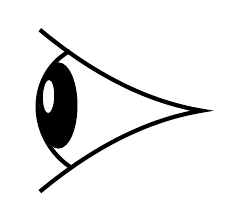
\begin{tikzpicture}[x=0.75pt,y=0.75pt,yscale=-1,xscale=1]
    \draw  [line width=1.5]  (300,100.33) .. controls (326,122) and (352,135) .. (378,139.33) .. controls (352,143.67) and (326,156.67) .. (300,178.33) ;
    \draw  [fill={rgb, 255:red, 0; green, 0; blue, 0 }  ,fill opacity=1 ] (308.94,116.33) .. controls (313.87,116.33) and (317.86,125.51) .. (317.85,136.83) .. controls (317.84,148.15) and (313.84,157.33) .. (308.91,157.33) .. controls (303.99,157.32) and (300,148.14) .. (300.01,136.82) .. controls (300.02,125.5) and (304.02,116.32) .. (308.94,116.33) -- cycle ;
    \draw  [draw opacity=0][line width=1.5]  (314.84,166.6) .. controls (311.87,164.64) and (309.14,162.18) .. (306.76,159.24) .. controls (295.12,144.82) and (296.6,124.33) .. (310.07,113.45) .. controls (311.48,112.32) and (312.96,111.33) .. (314.5,110.49) -- (331.14,139.55) -- cycle ; \draw  [line width=1.5]  (314.84,166.6) .. controls (311.87,164.64) and (309.14,162.18) .. (306.76,159.24) .. controls (295.12,144.82) and (296.6,124.33) .. (310.07,113.45) .. controls (311.48,112.32) and (312.96,111.33) .. (314.5,110.49) ;
    \draw  [fill={rgb, 255:red, 255; green, 255; blue, 255 }  ,fill opacity=1 ] (304.43,124.2) .. controls (306.09,124.25) and (307.32,128.01) .. (307.18,132.6) .. controls (307.05,137.19) and (305.59,140.88) .. (303.93,140.83) .. controls (302.27,140.78) and (301.03,137.02) .. (301.17,132.43) .. controls (301.31,127.83) and (302.76,124.15) .. (304.43,124.2) -- cycle ;
    \end{tikzpicture}
    }\,}

\newcommand{\um}[1]{\text{ #1}}
\newcommand{\sunmass}{M_{\astrosun}}
\newcommand{\inu}{I_\nu}
\newcommand{\anu}{\alpha_\nu}
\newcommand{\jnu}{j_\nu}
\newcommand{\snu}{\sigma_\nu}

\title{Appunti astrofisica}
\author{giac.nato }
\date{May 2021}

\begin{document}

\maketitle
\newpage
\section{Flusso di radiazione}
Energia del flusso: considerando un elemento di area $dA$ esposto alla radiazione per un tempo $dt$, la quantità di energia che attraversa l'elemento sarà proporzionale a $dAdt$. Scriviamo
\begin{equation}
    dE=F\,dA\,dt,
    \label{001}
\end{equation}
con $F$ flusso di energis, misurato in $\um{erg}\um{s}^{-1}\um{cm}^-2$.\\
Una sorgente di radiazione si dice isotropa quando emette energia in ugual modo in tutte le direzioni.
\begin{wrapfigure}{r}{0pt}
    \centering
    \resizebox{.3\columnwidth}{!}{%
        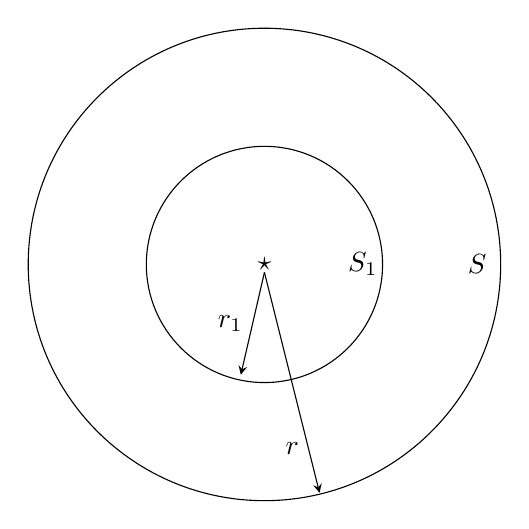
\begin{tikzpicture}
            \draw (0,0) circle (3);
            \draw (0,0) circle (1.5);
            \draw[-stealth] (0,-0.1) -- (-0.3,-1.4) node[left, pos=.5]{$r_1$};
            \draw[-stealth] (0,-0.1) -- (0.7,-2.9) node[left, pos=0.8]{$r$};
            \node(h1) at (1.25,0){$S_1$};
            \node(h2) at (2.7,0){$S$};
            \node(stella) at (0,0){$\star$};
        \end{tikzpicture}
    }
\end{wrapfigure}
 Un esempio è una stella sferica isolata. Ponendo due superfici immaginarie $S_1$ e $S$ con raggi $r_1$ e $r$, centrate nella stella, per la conservazione dell'energia sappiamo che l'energia ce passa attraverso $S_1$ è la stessa che passa attraverso $S$, quindi
\begin{gather*}
    F(r_1)\cdot 4\pi r_1^2\cdot dt = F(r)\cdot 4\pi r^2\cdot dt\\
    \Rightarrow F(r) = \frac{F(r_1)r_1^2}{r^2}.
\end{gather*}
Considerando $S_1$ fissa, abbiamo
\begin{equation*}
    F=\frac{\text{costante}}{r^2}.
\end{equation*}
Abbiamo quindi che il flusso di radiazione va come $1/r^2$.

%%%%%%%%%%%%%%%%%%%%%%%%%%%%%%%%%%%%%%%%%%%%%%%%%%%%%%%%%%%%%%%%%%%%%%%%%%%%%%%%%%%%%%%%%%%%%%%%%%%%%%%%%%%%%%%%%%%%%%%
\section{Intensità specifica}
Condisderiamo l'elemento di superficie $dA$, parte di una sorgente, orientato con $\hat{n}$ come in figura. 

\begin{figure}[h!]
        \centering
        \resizebox{0.5\columnwidth}{!}{
        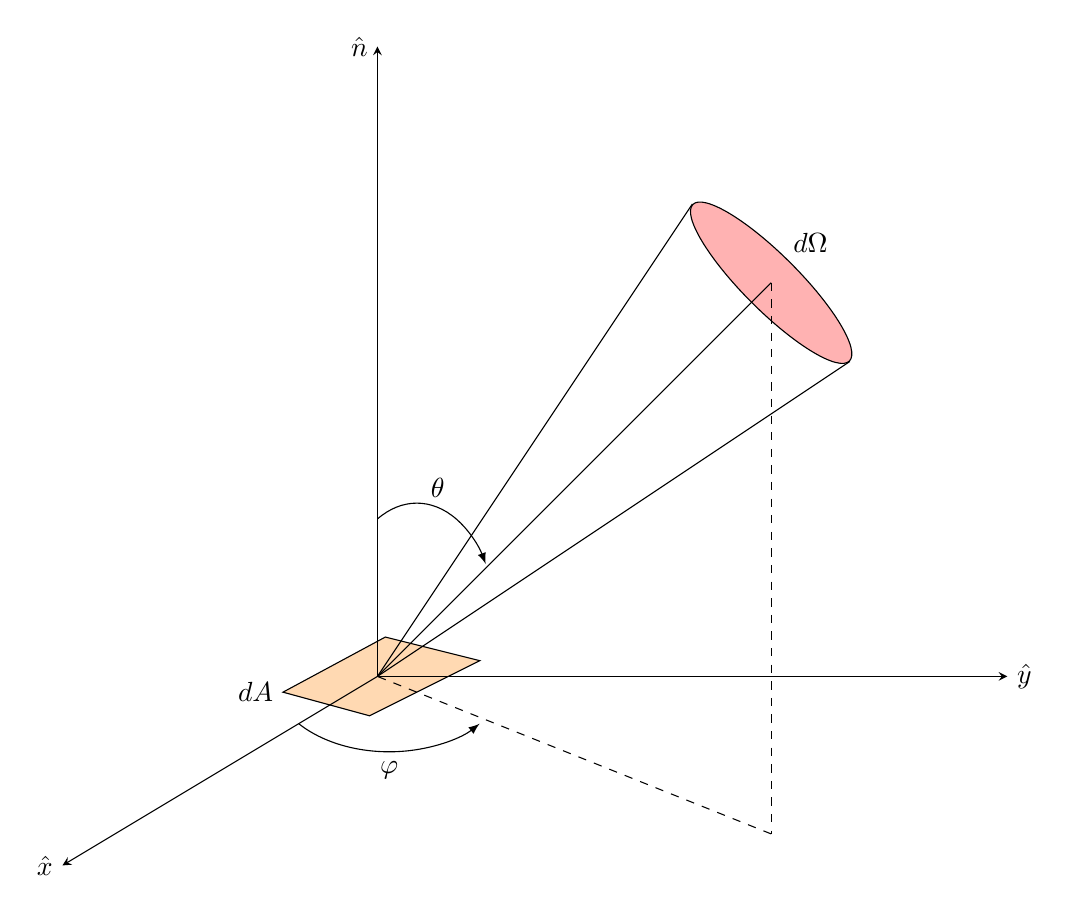
\begin{tikzpicture}
            \filldraw[fill=orange!30] (-1.2,-0.2) -- (0.1,0.5) -- (1.3,0.2) -- (-0.1, -0.5) -- cycle node[left, pos=1, color=black]{$dA$};
            \draw[-stealth] (0,0) -- (0, 8) node[left, pos=1]{$\hat{n}$};
            \draw[-stealth] (0,0) -- (8, 0) node[right, pos=1]{$\hat{y}$};
            \draw[-stealth] (0,0) -- (-4, -12/5) node[left, pos=1]{$\hat{x}$};
            \filldraw[rotate around={45:(5,5)},fill=red!30] (5,5) ellipse (10pt and 40pt);
            \node(ellips) at (5.5,5.5){$d\Omega$};
            \draw (0,0) -- (5,5);
            \draw (0,0) -- (6, 4);
            \draw (0,0) -- (4, 6);
            \draw[dashed] (5, 5) -- (5, -2);
            \draw[dashed] (5, -2) -- (0,0);
            \draw[-latex] (-1,-0.6) arc
                [
                    start angle=220,
                    end angle=320,
                    x radius=1.5cm,
                    y radius =1cm
                ] node[below, pos=0.5]{$\varphi$};
            \draw[-latex] (0,2) arc
                [
                    start angle=120,
                    end angle=29,
                    x radius=1cm,
                    y radius =1.5cm
                ] node[above, pos=0.5]{$\theta$} ;    
        \end{tikzpicture}
        }
\end{figure}
\noindent 
L'energia specifica (ad una certa frequenza) emessa in un tempo $dt$ da $dA$ nella banda $d\nu$ entro l'angolo solido $d\Omega$ è data da 
\begin{equation}
    dE_\nu \,d\nu=dE=\inu(\theta, \varphi)\cos\theta \,dA\,d\Omega \,d\nu\, dt
    \label{002}
\end{equation}
dove $\inu$ è detta intensità specifica (o radianza). Si misura in $\um{erg}\um{cm}^{-2}\um{s}^{-1}\um{ster}^{-1}\um{Hz}^-1$ o in $\um{W}\um{m}^{-2}\um{ster}^{-1}\um{Hz}^{-1}$.\\
$\inu$ dipende dalla posizione, dalla direzione e dalla frequenza. Nello stessa sistema della figura, il flusso a frequenza $\nu$ che passa dall'angolo solido $d\Omega$ (che quindi rispetto a \ref{001} riduce il flusso di un fattore $dA \cos\theta$) si scrive
\begin{equation*}
    dF_\nu=\inu \cos\theta\, d\Omega,
\end{equation*}
ed il flusso totale a frequenza $\nu$ sarà
\begin{equation*}
    F_\nu = \int \inu\cos\theta \,d\Omega,
\end{equation*}
che basterà integrare nelle frequenze per ottenere il flusso totale
\begin{equation*}
    F=\int F_\nu\, d\nu.
\end{equation*}
\paragraph{Nota:} Se $\inu$ fosse isotropa si avrebbe $F_\nu=0$ perché ci sarebbe uguale energia che attraversa con verso $\hat{n}$ e con verso $-\hat{n}$.\\
Per ottenere la quantità di moto per unità di area e di tempo (quindi la pressione) legata al flusso, normale rispetto a $dA$, basta ricordare che il momento del fotone è $p=E/c$, e di conseguenza il momento del flusso lungo un angolo $\theta$ sarà $F_\nu/c$. Per ottenere la componente lungo $\hat{n}$ basta moltiplicare per $\cos \theta$, così otteniamo
\begin{equation*}
    p_\nu = P_\nu = \frac{1}{c}\int\inu\cos^2\theta\, d\Omega
\end{equation*}

\section{Densità di energia radiativa}
Consideriamo l'energia in funzione della sua densità per unità di angolo solido
\begin{equation*}
    dE = u_\nu(\Omega)\,dV\,d\Omega\,d\nu.
\end{equation*}
Consideriamo un cilindro attorno ad un fascio con lunghezza $cdt$ e area $dA$.
\begin{figure}[h!]
        \centering
        \resizebox{0.5\columnwidth}{!}{
        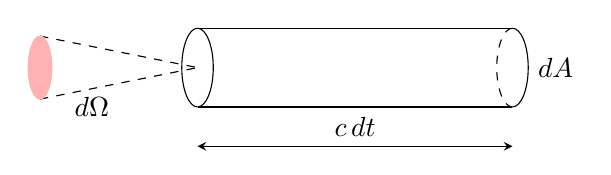
\begin{tikzpicture}
            \draw[dashed] (-1,0.9)--(1,0.5);
            \draw[dashed] (-1,0.1) -- (1,0.5);
            \filldraw[red!30] (-1,0.5) ellipse (0.15cm and 0.4cm) node[left, pos=0.5, black]{$d\Omega$};
            \draw (1,1) -- (5, 1);
            \draw (1,0) -- (5,0);
            \draw[stealth-stealth] (1, -0.5) -- (5, -0.5) node[above, pos=0.5]{$c\,dt$};
            \draw (1,1) arc
                [
                    start angle=90,
                    end angle=270,
                    x radius=0.2cm,
                    y radius =0.5cm
                ];
            \draw[dashed] (5,1) arc
                [
                    start angle=90,
                    end angle=270,
                    x radius=0.2cm,
                    y radius =0.5cm
                ];
            \draw (1,1) arc
                [
                    start angle=90,
                    end angle=-90,
                    x radius=0.2cm,
                    y radius =0.5cm
                ];
            \draw (5,1) arc
                [
                    start angle=90,
                    end angle=-90,
                    x radius=0.2cm,
                    y radius =0.5cm
                ] node[right, pos=0.5]{$dA$};
        \end{tikzpicture}
        }
\end{figure}
\\
Si ha che
\begin{equation*}
    dE=u_\nu(\Omega)\,dA\,c\,dt\,d\Omega\, d\nu.
\end{equation*}
Riscriviamo l'Eq. \ref{002} considerando $\theta=0$:
\begin{equation*}
    dE=\inu \,dA\,dt\,d\Omega\, d\nu.
\end{equation*}
Quindi ho che 
\begin{equation*}
    u_\nu(\Omega)=\frac{\inu}{c}.
\end{equation*}
Integrando nell'angolo solido si ottiene
\begin{equation}
    u_\nu = \frac{1}{c}\int\inu \,d\Omega = \frac{4\pi}{c}J_\nu,
    \label{003}
\end{equation}
in cui abbiamo definito l'intensità specifica media $J_\nu=\frac{1}{4\pi}\int\inu\, d\Omega$. \\
La densità di energia della radiazione totale si ottiene semplicemente integrando nella frequenza
\begin{equation*}
    u=\int u_\nu\,d\nu=\frac{4\pi}{c}\int J_\nu\,d\nu.
\end{equation*}
%%%%%%%%%%%%%%%%%%%%%%%%%%%%%%%%%%%%%%%%%%%%%%%%%%%%%%%%%%%
\section{Pressione di radiazione}
La pressione di radiazione su una superficie è data dal flusso del momento perpendicolare ad essa ($P=p/(dA\,dt)$). Come visto prima, il momento associato all'energia $dE_\nu$ vale $dE_\nu/c$ e a sua componente normale a $dA$ è $dE_\nu \cos\theta /c$. Dividendo per $dA\,dt$ otteniamo dalla \ref{002}
\begin{equation*}
    \frac{dE_\nu\,\cos\theta}{c\,dA\,dt}=\frac{\inu\cos^2\theta}{c}\,d\Omega.
\end{equation*}
Integrando in tutte le direzioni, la pressione di radiazione vale
\begin{equation*}
    P_\nu=\frac{1}{c}\int\inu\cos^2\theta\,d\Omega.
\end{equation*}
Se la radiazione è isotropa si ha
\begin{equation*}
    P_\nu=\frac{\inu}{c}\int\cos^2\theta\,d\Omega = \frac{4\pi}{3c}\inu\\
\end{equation*}
\paragraph{Nota:}
\begin{equation*}
    \int\cos^2\theta\,d\Omega=\int_0^{2\pi}\,d\varphi \int_0^\pi \cos^2\theta\sin\theta\,d\theta =2\pi\int_{1}^{-1}u^2(-du)=2\pi\left[\frac{u^3}{3}\right]_{1}^{-1}=\frac{4}{3}\pi
\end{equation*}
con $\cos\theta=u$ e $du=-\sin\theta\,d\theta$.\\
In caso di isotropia l'eq. \ref{003} diventa
\begin{equation*}
    u_\nu = \frac{\inu}{c}\int\,d\Omega = \frac{4\pi}{c}\inu,
\end{equation*}
Da cui otteniamo
\begin{equation*}
    P_\nu=\frac{u_\nu}{3}
\end{equation*}
per radiazione isotropa.
%%%%%%%%%%%%%%%%%%%%%%%%%%%%%%%%%%%%%%%%%%%%%%%%
\section{Costanza dell'intensità specifica lungo un raggio}
\begin{figure}[h!]
        \centering
        \resizebox{0.7\columnwidth}{!}{
        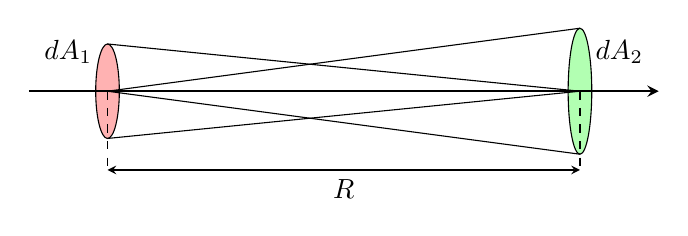
\begin{tikzpicture}
            \filldraw[fill=red!30] (-3,0.5) ellipse (0.15cm and 0.6cm);
            \filldraw[fill=green!30] (3,0.5) ellipse (0.15cm and 0.8cm);
            \draw[thin] (-3,1.1)--(3,0.5);
            \draw[thin] (-3,-0.1) -- (3,0.5);
            \draw[stealth-stealth] (-3, -0.5) -- (3, -0.5) node[below, pos=0.5]{$R$};
            \draw[thin] (-3,0.5)--(3,1.3);
            \draw[thin] (-3,0.5) -- (3,-0.3);
            \draw[thick,-stealth] (-4, 0.5) -- (4, 0.5);
            \draw[thin, dashed] (3,0.5) -- (3, -0.5);
            \draw[very thin, dashed] (-3,0.5) -- (-3, -0.5);
            \node at (-3.5,1) {$dA_1$};
            \node at (3.5,1) {$dA_2$};
        \end{tikzpicture}
        }
\end{figure}
Consideriamo due punti su un fascio e su ciascuno di essi costruiamo un'area, $dA_1$ e $dA_2$. Sfruttando la conservazione dell'energia scriviamo
\begin{equation*}
    dE_1 = I_{\nu_{1}}\,d\Omega_1\,dA_1\,d\nu_1\,dt_1 = dE_2 = I_{\nu_{2}}\,d\Omega_2\,dA_2\,d\nu_2\,dt_2.
\end{equation*}
$d\Omega_1$ è l'angolo solido sotteso da $dA_2$ a distanza $R$ dal punto in cui abbiamo costruito $dA_1$ e viceversa.\\
Dato che $d\Omega_1=dA_2/R^2$, $d\Omega_2=dA_1/R^2$, $d\nu_1=d\nu_2$ e $dt_1=dt_2$ si ha
\begin{gather*}
    I_{\nu_{1}}\,\frac{{dA_2}}{{R^2}}\,{dA_1}\,{d\nu\,dt} = I_{\nu_{2}}\,\frac{{dA_1}}{{R^2}}\,{dA_2}\,{d\nu\,dt}\\
    \Rightarrow I_{\nu_1} = I_{\nu_2} = I_\nu.
\end{gather*}
Quindi lungo un fascio, $\inu$ è costante.\\
Vogliamo mostrare che la costanza di $\inu$ e la legge dell'inverso del quadrato della distanza non sono in conflitto. Consideriamo la seguente situazione:
\begin{figure}[h!]
        \centering
        \resizebox{0.7\columnwidth}{!}{
        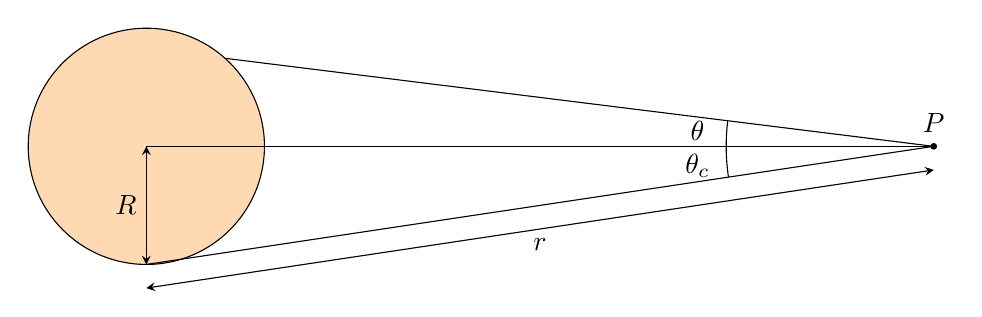
\begin{tikzpicture}
            \filldraw[fill=orange!30] (0,0) circle (1.5);
            \draw[stealth-stealth] (0, 0) -- (0, -1.5) node[left, pos=0.5]{$R$};
            \draw (0, 0) -- (10, 0);
            \filldraw [black] (10,0) circle (1pt);
            \draw (0,-1.5) -- (10,0); 
            \draw (1, 1.118) -- (10,0);
            \node at (10, 0.3) {$P$};
            \draw[stealth-stealth] ( 0, -1.8) -- (10,-0.3) node[below, pos=0.5]{$r$};
            \path[clip] (0,-1.5) -- (10,0) -- (0,1.24) -- cycle;
            \node[circle,draw=black,minimum size=150pt] at (10,0) (circ) {};
            \node at (7,-0.25) {$\theta_c$};
            \node at (7,0.2) {$\theta$};
        \end{tikzpicture}
        }
\end{figure}
calcoliamo il flusso di una stella che abbia intensità specifica uniforme $B$. \'E una sorgente isotropa, quindi al punto $P$ l'intensità sarà
\begin{equation*}
    I(P)=
    \begin{cases}
    B,\quad 0<\theta<\theta_c\\
    0,\quad \theta>\theta_c
    \end{cases}
\end{equation*}
con $\theta_c =\arcsin\frac{R}{r}$. Calcolando il flusso abbiamo
\begin{align*}
    F=\int I\cos\theta\,d\Omega &= B\int_{0}^{2\pi}\,d\varphi\int_{0}^{\theta_c}\cos\theta\sin\theta\,d\theta =\\
    &=2\pi B\int_{0}^{\cos\theta_c}-u\,du=\\
    &=\pi B(1-\cos^2\theta_c)=\\
    &=\pi B \sin^2\theta_c=\\
    &=\pi B \frac{R^2}{r}.
\end{align*}

\section{Trasporto radiativo}
Quando un fascio passa attraverso la materia, l'energia può essere fornita o sottratta per assorbimento ed emissione, ed in generale l'intensità specifica non resterà costante.
\subsection{Emissione}
Il coefficiente di emissione spontanea $j$ è definito come l'energia emessa per unità di tempo, per unità di angolo solido e per unità di volume
\begin{equation*}
    dE = j\,dt\,d\Omega\,dV.
\end{equation*}
Il coefficiente di emissione monocromatico si definisce analogamente
\begin{equation*}
    dE_\nu\, d\nu = dE = j_\nu\, dt\, d\Omega\,dV\,d\nu,
\end{equation*}
in cui $j_\nu$ ha le unità di $\um{erg}\um{s}^{-1}\um{ster}^{-1}\um{cm}^{-3}\um{Hz}^{-1}$.\\
Percorrendo una distanza $ds$, un fascio con sezione $dA$ attraversa un volume $dV=dA\,ds$. Quindi l'intensità aggiunta al fascio per emissione sèpntanea è
\begin{equation}
    d\inu = j_\nu\,ds.
    \label{004}
\end{equation}

\subsection{Assorbimento}
Definiamo il coefficiente di assorbimento, $\anu$ ($\um{cm}^{-1}$), con la seguente equazione, che rappresenta la perdita di intensità in un raggio che percorre una distanza $ds$
\begin{equation}
    d\inu=-\anu\inu\,ds
    \label{005}
\end{equation}
(per convenzione $\anu$ è positivo quando il raggio perde energia). Questa legge fenomenologica può essere compresa in termini di un modello microscopico in cui particelle con densità $n$ (numero di particelle per unità di volume) hanno ognuna una sezione d'urto $\snu$. Si assume che le particelle siano distribuite casualmente. Consideriamo gli effetti di questi assorbitori sulla radiazione attraverso $dA$ entro un angolo solido $d\Omega$.
\newpage
\section*{26-04 - Nascita di una stella}
In seguito all'instabilità di Jeans, le nubi cominciano a collassare sotto l'effetto della gravità. Succede che il raggio diminuisce e aumenta la densità della nube, inizialmente molto rarefatta, fino a che la materia non diventa fortemente opaca e intrappolando la radiazione al suo interno si scalda. Parte della materia forma un disco di accrescimento (dovuto ad una piccola rotazione che poi viene amplificata). Man mano che il tempo passa il disco viene in parte spazzato via e con quello che resta si formano pianeti e sistema planetario. Abbiamo delle conferme guardando nella regione più profonda della nebulosa di Orione. Nel visibile non riusciamo a penetrarla ma nell'infrarosso notiamo la presenza di stelle molto giovani, immerse ancora nella nube da cui sono nate. Non c'è ancora stato il tempo per spazzarla via. Grazie al HST sono stati scoperti i primi dischi protoplanetari. (pag. 19/83 evoluzione-stellare) \\
Cosa succede alla stella? Una volta spazzato via il gas, la stella si troverà in una condizione di grande espansione e di $T_{\text{eff}}$ relativamente bassa. In un diagramma HR si trova nella regione in alto a destra (alta luminosità e bassa temperatura). Questa zona prende il nome di presequenza principale. (pag. 28/83). Si evolve col teorema del viriale, con tempi scala di Kelvin Helmoltz, contraendosi e aumentando la propria temperatura. Quando arriverà alla temperatura intorno al milione di gradi, verrà bruciato il deuterio ($p+d$) prima di iniziare la $p+p$. Questa fase dura poco e vediamo che nel diagramma HR la traccia verticale subisce una piccola deviazione. In che condizione si trova la stella nella fase verticale? Bassa temperatura effettiva: gran parte degli atomi di idrogeno nell'atmosfera esterna sono neutri o parzialmente ionizzati, quindi abbiamo un inviluppo in una situazione di instabilità convettiva: viene violato il criterio di Schwarzschild (l'opacità è alta, aumenta il gradiente radiativo che supera quello adiabatico e quindi viola il criterio). Quindi nella fase verticale tutta la stella è convettiva e di conseguenza chimicamente omogenea. La traccia verticale si chiama Traccia di Hayashi. Essa è una sorta di confine, nel senso che non esistono strutture all'equilibrio idrostatico per una stella di data massa a destra della traccia. \\
Sappiamo che al crescere della temperatura l'opacità diminuisce (legge di Kramers) e quindi non viene più violato il criterio di Schwarzschild. Si creerà quindi una zona radiativa nel punto più caldo, nel centro. Quando si sviluppa un nucleo radiativo, la stella si allontana dalla fascia di Hayashi e si raggiungono temperature per innescare $p+p$. All'inizio gli elementi secondari (deuterio, elio, ...) non sono all'equilibrio. Quando anche questi raggiungono l'equilibrio la stella si posiziona nel punto di ZAMS (Zero Age Main Sequence). Da quel momento in poi inizia la fase di sequenza principale (combustione centrale dell'idrogeno). Per una stella come il Sole la presequenza dura 30 milioni di anni, mentre la fase di sequenza principale dura circa 10 miliardi di anni. Naturalmente stelle di massa diversa avranno durate diverse. (pag. 29/83). Cambia il rapporto tra zona orizzontale e zona verticale. Più grande è la massa e meno tempo starà sulla fascia di Hayashi, perché sono più calde. \\
Riassumendo: fase vericale struttura convettiva, zona orizzontale core radiativo, poi si posiziona sulla sequenza principale.
\newpage
\section*{29-04 - Evoluzione stellare}
Illustreremo le principali fasi evolutive della stragrande maggioranza delle stelle. \\
Guardando un'immagine del Sole (nell'UV) notiamo una granularità dovuta ai moti convettivi. Nell'inviluppo (parte esterna) è instabile convettivamente, viene violato il criterio di Schwarzschild. Il motivo è riconducibile all'alta opacità della zona. Nel caso del Sole questo inviluppo si estende per circa il $30\%$ del raggio. Mentre le zone centrali sono all'equilibrio radiativo (core all'equilibrio). Non tutte le stelle sono fatte così. La distinzione principale dipende dalla massa, che risulta il parametro dominante per le caratteristiche principali delle stelle. Conta anche la composizione chimica ma meno. Studiando le reazioni nucleari abbiamo visto che abbiamo due canali: $pp$ e $\ce{CNO}$. Quest'ultima ha bisogno di temperature più alte. La dipendenza della temperatura nella produzione di energia nucleare è molto più spinta nella $\ce{CNO}$: $pp$ va come $T^4$, $\ce{CNO}$ come $T^{15}$. Per masse abbastanza piccole (tra $0.4M_{\astrosun}$ e $1.2M_{\astrosun}$), in sequenza principale non si ha temperatura abbastanza alta per avviare la $\ce{CNO}$ e si ha quindi $pp$ che avviene nel core. Ma nelle stelle abbastanza calde ($T_c\approx 15\times10^6$, e di conseguenza massicce($>1.2M_{\astrosun}$)), la $\ce{CNO}$ diventa poi domninante. Quindi nelle stelle abbastanza piccole, in cui avviene solo $pp$ nel core, quest'ultimo è all'equilibrio radiativo perché il flusso non è sufficientemente intenso da far diventare $\nabla_{rad} > \nabla_{ad}$. Nelle stelle sufficientemente grandi avviene $\ce{CNO}$, e alle temperature alle quali si ha questo tipo di produzione spostandosi dal centro verso l'esterno ci sarà una variazione molto brusca come produzione di energia nucleare, che sarà molto più concentrata nel core. Ciò fa sì che si abbia un flusso molto più intenso che fa crescere il $\nabla_{rad} > \nabla_{ad}$. Da notare come una proprietà microscopica (efficienza di produzione $\ce{CNO}$ rispetto a $pp$) ha un effetto macroscopico. Per quanto riguarda l'inviluppo invece si ha la situazione opposta: le stelle piccole hanno inviluppo convettivo, quelle grandi inviluppo radiativo. Le stelle più piccole hanno l'inviluppo convettivo poiché la zona è più fredda con temperature alle quali c'è una parziale ionizzazione (che implica alta opacità). Le stelle più grandi sono abbastanza calde da avere l'inviluppo completmaente ionizzato. La massa che discrimina questi due comportamenti è circa $1.2M_{\astrosun}$. \\
Scendendo ancora in massa (0.4-0.3 masse solari), succede che la stella diventa completamente convettiva. L'inviluppo convettivo affonda sempre di più fino a coprire l'intera struttura. (pag38/83 evoluzione-stelle). \\
Sappiamo che i moti convettivi avvengono con tempi scala molto brevi rispetto al tempo scala nucleare. Quindi ci aspettiamo che le regioni convettive siano chimicamente omogenee (pag 40/83 ma spiegano bene la cosa i grafici a pag. 4 e 47.). Come mai ci fermiamo ad una massa di $(0.09\div0.08)M_{\astrosun}$? Perché la stella, se non ha sorgenti nucleari attive, si contrae in risposta alla perdita di energia per luminosità, quindi aumenta la temperatura centrale e aumenta la densità. Può succedere che prima che la stella raggiunga le temperature necessarie per la combustione dell'idrogeno, la stella raggiunge densità sufficienti per la configurazione di degenerazione elettronica. Per masse minori di $0.08\sunmass$ la stella degenera prima di iniziare a bruciare l'idrogeno. Al posto di una stella si viene a creare una Brown Dwarf (Nana bruna), che è una via di mezzo tra una stella ed un pianeta.\\
Sappiamo che una relazione importante è quella massa luminosità $L\propto M^3$. A pag 42 abbiamo i risultati esatti, ed effettivamente in certi range di masse si ha un andamento a legge di potenza con una potenza che varia intorno a 3.\\
Una volta che la stella è in sequenza principale brucia l'idrogeno con i secondari all'equilibrio. Man mano che passa il tempo finirà l'idrogeno nel centro e di conseguenza anche la fase principale. A seconda della massa della stella, si avrà un'evoluzione diversa. (pag. 44/83). La stella si sposta a temperature più alte (sx) e poi aumenta la sua luminosità (alto). A quel punto la traccia curva verso destra, diminuendo quindi la temperatura. Il punto in cui ciò avviene prende il nome di \textit{Turn Off}. In quel punto si ha la temperatura effettiva più alta e corrisponde al momento in cui l'idrogeno finisce. Questa curva è molto dolce, dato che l'idrogeno finisce prima al centro e si deve spostare ad una shell. Il core è quindi diventato di elio, circondato da una shell di idrogeno che brucia. Le stelle che bruciano con $\ce{CNO}$ non hanno lo stesso andamento, ma hanno un andamento a zig zag che prende il nome di \textit{overall contaction} (pag 46/83) ed è dovuta al fatto che la combustione avviene in una zona convettiva. Infatti l'idrogeno non viene bruciato solo al centro, ma in tutta la zona in cui c'è convezione. Questa zona è più grande della zona in cui ci sono le temperature necessarie per bruciare l'idrogeno, quindi quando quest'ultimo termina e si crea il core di elio, nella shell successiva la temperatura non è abbastanza alta per innescare la combustione dell'idrogeno (pag. 47/83). Di conseguenza non si ha il passaggio dolce dal core alla shell, quindi la stella contrae con tempi scala di KH e si ha l'andamento a zig zag. Vediamo come varia il tempo di vita in funzione della massa nel grafico a pag 58/83. \\
Il core della stella appena uscita dalla sequenza principale è formato da elio. Per innescare la $3\alpha$ ci vogliono centinaia di milioni di gradi, quindi in questa fase il core è inerte poiché non ci sono le temperature adeguate perché la reazione avvenga. Attorno al core abbiamo una shell in cui brucia l'idrogeno con temperature abbastanza elevate perché avvenga il $\ce{CNO}$. Attorno alla shell abbiamo l'inviluppo. Quando si accende la shell di idrogeno, l'inviluppo si espande moltissimo aumentando il raggio della stella di qualche ordine di grandezza (nel caso del sole di circa 100 volte). La stella diventa quindi una gigante rossa, il cui core è molto piccolo in raggio, molto molto denso, mentre si ha un enorme inviluppo estremamente rarefatto. Quando il sole diventerà una gigante rossa, nel core di elio si avranno densità dell'ordine del milione di grammi per centimetro cubo mentre la densità in una zona media dell'inviluppo sarà minore di quella dell'aria che respiriamo. La shell di idrogeno produce elio che nel tempo fa aumentare la massa del core. Quindi nella fase di gigante rossa, la combustione nucleare è solo in shell e questa combustione determina un progressivo aumento della massa del core di elio (struttura a pag. 51/83). L'inviluppo sarà convettivo. Cosa fa nel diagramma HR? Uscita dalla sequenza principale, passa dal turn off e va verso destra \textit{(fase di sub gigante}) e poi sale a luminosità progressivamente più alte (\textit{ramo delle giganti rosse}). Nel ramo delle giganti rosse il core si sta riscaldando, fino al punto in cui non si arriva alle temperature che inneschino la combustione centrale dell'elio, la $3\alpha$. Questo innesco può avvenire in due modi distinti a seconda della massa della stella. Per masse non troppo grandi ($<2.3\sunmass$) il core di elio diventa degenere in gigante rossa. Per stelle di massa più grande il core non è degenere. Noi sappiamo che un mezzo degenere si comporta in maniera diversa rispetto ad uno non degenere in risposta all'innesco di una reazione nucleare. Prendiamo una situazione non degenere: accendendo le reazioni termonucleari si libera energia, aumenta la temperatura e, siccome il mezzo non è degenere, aumenta la pressione e la regione risponde espandendosi e quindi diminuisce la temperatura. C'è un effetto che tende a calmare l'innesco e si raggiunge una situazione di equilibrio. Viceversa, in un mezzo degenere sappiamo che la pressione è largamente dominata dalla pressione degli elettroni degeneri, ma in quel caso la dipendenza dalla temperatura è praticamente assente. Quindi nel momento in cui inneschiamo la reazione termonucleare liberiamo energia, aumenta la temperatura ma, dato che la pressione non dipende dalla temperatura per un mezzo degenere, la regione non si espande e tutta l'energia liberata fa aumentare la temperatura, aumenta quindi il rate delle reazioni nucleari e abbiamo un meccanismo che si autoincentiva. Questo meccanismo si chiama \textit{flash dell'elio} ed è ciò che succede in stelle che hanno una massa inferiore a $2.3\sunmass$. Il vertice del ramo delle giganti rosse è in corrispondenza del flash dell'elio. Viene liberata un'enorme energia che non porta alla distruzione della stella ma alla rimozione della degenerazione. Nelle stelle di massa più grande invece, il core non è degenere, l'innesco avviene in maniera più controllata ed a luminosità più basse perché il core, non essendo degenere, si scalda più facilmente. In entrambi i casi, come risultato si ha che la stella passa in una fase evolutiva in cui si avvia la combustione dell'elio nel core. Abbiamo quindi due sorgenti di energia nucleare: il core di elio e la shell di idrogeno. La combustione dell'elio avviene in un core convettivo, poiché la dipendenza dalla temperatura della $3\alpha$ è molto grande ($\sim T^{40}$). (Approfondire cosa succede nel diagramma HR durante la combustione dell'elio). Finita la combustione dell'elio si ha la fase di \textit{Ramo Asintotico Gigante (AGB)} in cui si ha il passaggio dalla combustione in core alla combustione in shell dell'elio, attorno ad un core inerte costituito da $\ce{C}$ e $\ce{O}$  (pag. 60/83). Il Sole passerà per quetsa fase evolutiva, alla fine della quale non riuscirà ad innescare la combustione del core C-O. Man mano che la combustione in fase AGB (Asymptotic Giant Branch) procede, il core C-O aumenta in massa e ci troviamo di fronte ad una biforcazione: riuscirà la stella ad innescare C-O? Dipenderà dalla massa ($8\sunmass$ è la frontiera). Ad esempio il sole non ce la farà. Ciò che succede nel caso non si riesca è (pag. 62/83) la stella sale nel HR, non innesca C, l'inviluppo sarà molto molto rarefatto e la stella perderà molta massa per via dei venti solari fino a che, non riuscendo a innescare il C, comincerà a contrarsi e aumenterà la temperatura fino a diventare una \textit{Nana Bianca}. Quest'ultima si evolve nel diagramma HR lungo una traccia diagonale che implica il raggio costante della stella. Per capirlo basta considerare la relazione 
\begin{equation*}
    L = 4\pi R^2\sigma T_{\text{eff}}^4
\end{equation*}
Quindi vediamo come la luminosità sia legata a raggio e temperatura. Avendo nel nostro piano $\log L$ e $\log T_{\text{eff}}$ abbiamo
\begin{equation*}
    \log L = \log(4\pi R^2\sigma T_{\text{eff}}^4)
\end{equation*}
e abbiamo quindi una retta che è a raggio costante. \\
Nel passaggio dalla zona fredda a quella calda la radiazione elettromagnetica emessa dalla stella diventa tale da ionizzare il gas costituito dai venti stellari emessi precedentemente. Questa fase, molto bella, prende il nome di \textit{nebulosa planetaria}. (pag. 64/83) La materia diffusa che osserviamo è l'inviluppo eroso dai venti solari precedentemente che poi viene riscaldata e di conseguenza ionizzata. Si chiama così per motivi storici ma non hanno nulla a che vedere con i pianeti.\\
Le stelle di grande massa ($>8\sunmass$ e quindi che innescano C), se hanno massa >10 masse solari riescono ad innescare tutte le reazioni nucleari successive. Riusciranno quindi ad attraversare tutte le fasi di combustione fino ad arrivare alla combustione del silicio per produrre un nucleo di ferro inerte. (pag. 74/83) Si verrà a formare una struttura a cipolla, dovuta al fatto che l'estensione della regione in cui brucia un elemento sarà più piccola di quella in cui è bruciato l'elemento precedente. Arrivati a quel punto la stella non produrrà più energia con reazioni di fusione nucleare e quello che succederà è che, quando il core di elio diventa abbastanza grande, la stella diventa instabile (instabilità dovuta alla forte degenerazione elettronica del core di ferro, si ha densità così elevata da avere un'energia di fermi di questi elettroni così elevata da innescare i processi beta inversi - lo vedremo -, e sottraendo gli elettroni la pressione diminuisce e quindi inizia un collasso molto rapido (frazione di secondo)). Si arriverà ad una stella di neutroni o buco nero per il nucleo ed il resto verrà eiettato con un'esplosione di supernova (pag. 75/83).
\newpage
\section*{03-05 - Diagrammi HR di Ammassi e Stelle di campo}
Uno dei diagrammi più importanti dell'astrofisica è il diagramma Hertzsprung - Russell (HR). Ha sull'asse delle ordinate una quantità legata alla luminosità, la magnetudine. Sulle oscisse avremo la controparte osservativa della temperatura effettiva: indice di colore o il tipo spettrale. 
\subsection*{Ammassi aperti}
Vediamo (a pag 2/49 HR) delle sequenze diverse. I primi due sono diagrammi di due ammassi (Pleiadi e Iadi), mentre il terzo sono stelle di campo vicine al sole. Dove sta la differenza? I primi due sono oggetti che nascono dalla stessa nube, quindi con composizione chimica molto simile, e ad un tempo simile (le stelle sono coeve). Queste condizioni rendono gli ammassi stellari dei laboratori di astrofisica che permettono la verifica dei modelli. In particolare le Pleiadi appartengono alla categoria degli ammassi aperti. Analizzando il diagramma HR delle Pleiadi notiamo che le stelle si dispongono sulla sequenza principale. Sappiamo quindi che sono stelle che bruciano idrogeno nel core. Ciò che differenzia queste stelle è la massa, che sappiamo essere proporzionale a luminosità e alla temperatura effettiva. Vediamo che a destra della sequenza principale si dispongono delle stelle. Sono binarie non risolte! Quindi la magnitudine che misuriamo, pensiamo che sia quello di una singola stella, ma in realtà è quella di una coppia. Guardando invece il diagramma delle Iadi, osserviamo una sequenza monoparametrica (cambia solo la massa). Vediamo, a differenza che per le Pleiadi, una parte superiore in cui è presente una curva, differenza dovuta all'età dell'ammasso. Esiste anche una differenza in composizione chimica, ma è un effetto secondario rispetto all'età. Guardando la figura a pag. 13/39, come si spiega che l'ammasso NGC 2362 ha una sequenza principale che arriva a luminosità molto più alte rispetto a M67? Abbiamo visto che per le stelle in sequenza principale il tempo di vita decresce al crescere della massa. \\
Per vedere come cambia la posizione di una stella a massa fissata in un diagramma HR teorico, abbiamo quelle che si chiamano tracce evolutive (pag. 15/49). Qual è la controparte teorica di un diagramma HR evolutivo di un ammasso? Non è la traccia evolutiva ma è l'isocrona (pag. 16/49). Non è altro che il luogo dei punti che hanno stessa età, stessa composizione chimica iniziale ma masse diverse. Guardando la figura, ci rendiamo conto che il turn off sia un ottimo indicatore di età. \'E lo strumento teorico che ci permette di datare i sistemi stellari. Uno prende le isocrone teoriche, le posiziona sul diagramma osservativo e si fa un fit.\\
Forma non ben definita, difficilmente superano qualche migliaio di stelle, range ti età molto vasto.
\subsection*{Ammassi globulari}
Il termine globulare viene dalla caretteristica simmetria sferica. Hanno tra alcune decine di migliaia fino a milioni di stelle. Sono tutti vecchi, nella nostra galassia non esistono ammassi globulari giovani (hanno età maggiori di $10^{10}$ anni) e sono per questo fondamentali per conoscere le fasi iniziali della galassia. Ci aspettiamo che la loro composizione chimica sia diversa rispetto agli ammassi più giovani, infatti sono poveri di metalli. Essendo così antichi ci aspettiamo anche che la sequenza principale sia molto più corta (pag. 20/49). C'è voluto molto tempo per riuscire a risolvere le singole stelle dell'ammasso perché mediamente sono molto lontani da noi ($2\um{kpc}$ il più vicino). In sequenza principale avremo stelle con luminosità più bassa e magnitudine apparente più grande. Inoltre nelle immagini c'è il problema dell'affollamento (crowding). Una grossa differenza nei diagrammi HR è che i globulari hanno un vistoso ammasso delle giganti rosse ed un ramo orizzontale che negli aperti non abbiamo visto. Quest'ultimo è molto "orizzontale" e molto esteso perché le stelle hanno, nel ramo di giganti rosse, perché perdono massa in modo stocastico. \\
A differenza degli ammassi aperti, negli ammassi globulari abbiamo popolazioni di stelle con età diversa e diversa composizione chimica.
\subsection*{Stelle di campo}
Guardando un diagramma di stelle di campo notiamo una grande dispersione (pag. 34/49). Continuiamo a vedere le fasi principali ma osserviamo una sequenza principale molto più larga, analogamente nel ramo delle giganti. Il motivo è proprio dettato dal fatto che queste stelle sono il risultato di molte generazioni distinte di stelle, con età e composizioni chimiche molto diverse. La DR2 di GAIA ha rivoluzionato anche questo diagramma (pag. 38/49). Si riescono a parallassare distanze maggiori e vedere stelle a grandi magnitudini. Notiamo che aumenta la larghezza della sequenza principale e che compaiono parti che prima non vedevamo, come la sequenza delle nane bianche.\\
Se non abbiamo l'informazione sulla parallasse vediamo una situazione molto più complicata (pag. 40/49). Abbiamo a che fare con le magnitudini apparenti, quindi una stella ci può sembrare più luminosa di un'altra nonostante non lo sia, semplicemente perché più vicina a noi, ed il diagramma diventa molto più difficile da interpretare. \\

\section*{Galassie nane}
A pag 41/49 vediamo un primo esempio di una galassia nana. È una galassia satellite della via lattea e dista $\sim 140\um{kpc}$ da noi. I puntini che vediamo non sono stelle ma ammassi globulari di questa galassia. Fino a poco tempo fa non riusciva a costruire un diagramma HR di questa galassia poiché la distanza era tale da non riuscire a risolverne le stelle. Col HST siamo riusciti a risolverle. Notiamo alcune differenze (pag. 43/49): non vediamo la sequenza principale, perché è molto lontano. Con un'integrazione maggiore si sarebbe potuta vedere una parte più bassa. E' fondamentale rendersi conto del fatto che l'universo è garnde e non riusciamo a risolvere stelle troppo lontane o non abbastanza luminosa. Tornando al diagramma, notiamo che ci sono più fasi evolutive. Si capisce perché notiamo sia una parte abbastanza giovane di sequenza principale, sia il ramo delle giganti rosse. 

\section*{Binarie}
(Pag. 45/49) Immaginiamo di avere due stelle che orbitano attorno al comune centro di massa. Immaginiamo di non riuscire a risolverle. Riusciamo ad accorgerci che siano una coppia guardando gli spettri e analizzando l'effetto Doppler che, a differenti tempi, farà sì che si abbiano spettri diversi. In questo caso si parla di \textit{Binarie spettroscopiche}. Se il piano dell'orbita è lungo la linea di vista, succede che le due stelle periodicamente passino una d'avanti all'altra. Nonostante non siamo in grado di risolvere questa coppia, osserviamo una variazione della luminosità del puntino. Parliamo di \textit{Binarie ad eclisse} (pag. 46/49). Quindi ci rendiamo conto che questo è un sistema binario con strumenti fotometrici. Le binarie ad eclisse sono molto interessanti poiché sono gli unici sistemi per i quali si riesce a dare una misura precisa e accurata di massa. Se uno riuscisse a misurare anche gli spettri, quindi misura delle velocità radiali, riuscirebbe a misurare anche il raggio. Sono quindi oggetti che riescono a vincolare i modelli teorici. Un'altra tipologia di binarie è quella di \textit{Binarie astrometriche} nelle quali si fanno misure, appunto, astrometriche cioé di posizione nel cielo. A pag. 48/49 vediamo una misura del moto proprio della stella Sirio (spostamento nella direzione ortogonale alla direzione di vista). Questa immagine è ciò che ha permesso a Bessel di capire, un paio di secoli fa, che Sirio non sia una stella singola ma appartiene ad un sistema binario. E vedremo che la compagna di Sirio, Sirio B, è stato il primo esempio di nana bianca.
\newpage
\section*{05-13 - Supernovae}
Una volta scoperto il neutrone nel 1932 ci sono voluti pochi anni dalla prima predizione dell'esistenza delle stelle di neutroni. Nel 1933 W. Baade e F. Zwicky suggeriscono l'esistenza di oggetti così compatti da essere fatti soltanto da neutroni. In quel periodo studiavano le supernovae, alcuni tra i processi più energetici del cosmo e per giustificare l'energia emessa da questi oggetti suggerirono che questa energia provenisse dal collasso gravitazionale del core di una stella massiccia che passa dalle dimensioni tipiche del core di una stella massiccia a quelle di una stella di neutroni. Proprio nell'articolo pubblicato suggeriscono che le densità che si vengono a trovare siano confrontabili con quelle dei nuclei atomici. Sempre nel 1934 Chandrasekhar insieme a von Neumann riscrivono le equazioni dell'equilibrio idrostatico tenendo conto della relatività generale proprio per descrivere la fisica di oggetti così compatti. Non pubblicheranno questo risultato che verrà poi reso pubblico nel 1939 da Tolman - Oppenheimer e Volkov indipendentemente.\\
Per i decenni successivi ci si dimentica delle stelle di neutroni, che non erano altro che speculazioni teoriche. La prima evidenza sperimentale risale al 1967/68 quando viene scoperta la prima pulsar.\\
L'11 Novembre 1572 nella costellazione di Cassiopea è comparsa una nuova stella, talmente brillante da avere luminosità apparente simile a quella di Giove. Uno dei più grandi studiosi di questo evento fu Tycho Brahe. Egli provò a misurarne la parallasse, che però risultò inferiore alla risoluzione dello strumento, il che implicò che l'oggetto dovesse essere oltre la sfera della Luna, cosa che determinò la crisi del modello per il quale oltre questa sfera tutto fosse immutabile. Oggi sappiamo che quella non era una stella ma una supernova, la supernova di Tycho (SN 1572). Oggi vediamo i resti dell'esplosione, e vediamo gli strati che si stanno espandendo a migliaia di km al secondo. Sappiamo che corrisponde ad un particolare tipo di supernova, le SN Ia e corrisponde all'esplosione di una nana bianca che ha superato la $M_{Ch}$.
\subsection*{Classificazione SN}
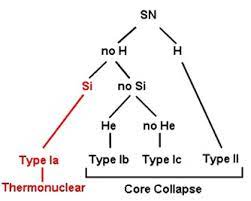
\includegraphics{images/snclass.jpg}
La prima classificazione si bassa sullo studio dello spettro. La prima biforcazione compara la  presenza di $\ce{H}$. Se è presente sono di tipo II altrimenti di tipo I. Se tra le I è presente il Si, allora si parla di tipo Ia, altrimenti si passa a valutare la presenza di He: se è presente sono le Ib, altrimenti Ic. Le Ia sono chiamate termonucleari, mentre le altre sono chiamate Core Collapse. Ci rendiamo quindi conto che le II, Ib e Ic hanno come progenitore una stella massiccia ($M.9.5\sunmass$). La differenza tra questi tre casi è nella parte più esterna. Le tipo II hanno avuto una perdita di massa che non ha eroso lo strato più esterno ricco di H. Se la perdita di massa è abbastanza efficiente da erodere tutto l`inviluppo esterno prima che la stella esploda non abbiamo più idrogeno nel momento dell'esplosione. Quindi la differenza sta nell'efficienza della perdita di massa prima che la stella esploda.
\subsubsection*{Instabilità}
Abbiamo la struttura del core a cipolla, con un core di ferro circondato dalla shell in silicio e via dicendo. Sappiamo che il core è il risultato della combustione del silicio da cui viene prodotto il ferro. Perché a quel punto diventa instabile? Sappiamo che la shell di silicio è attiva, quindi bruciando produce ferro che fa aumentare la massa del core. Quindi il core è elettronicamente degenere, inerte e aumenta in massa. È come se avessimo una nana bianca dentro la stella massiccia. Ciò implica che la sua massa non può aumentare a piacere poiché esiste il limite di Chandrasekhar. Facendo il calcolo, sappiamo che $\mu_e\approx2.15$ che sostituito nella formula della massa limite otteniamo $M_{Ch}\approx 1.25\sunmass$. Quindi quando il core raggiunge questa massa si ha un'instabilità. Si attiveranno i processi di cattura elettronica
\begin{equation*}
    (A,Z)+e^- \to (A, Z-1)+\nu_e
\end{equation*}
Sappiamo che la pressione è dominata dalla pressione degli elettroni degeneri. Questo processo, sottraendo elettroni, sottrae pressione. Ci aspettiamo quindi che l'equilibrio idrostatico non sia soddisfatto ed inizia il collasso del core. Durante il collasso aumenta la densità, quindi l'energia degli elettroni degeneri, il che amplifica il processo di cattura elettronica. Nel collasso inoltre il core si sta scaldando e una volta raggiunte $T\approx (6\div7)\times10^9$ i fotoni fotodisintegrano i nuclei di ferro producendo elio:
\begin{equation*}
    \ce{{}^{56}Fe +{\gamma}  -> 13{}^{4}He +4n}
\end{equation*}
Per ogni nucleo di ferro, questo processo sottrae $100$ MeV. Stiamo facendo il percorso opposto a quello di una stella, tornando indietro nel diagramma di energia di legame vs numero di massa, sottraendo energia alla stella, fino a quando non si raggiunge la temeperatura che fotodisintegra i nuclei di elio:
\begin{equation*}
    \ce{^{4}He + {\gamma} -> 2p + 2n}
\end{equation*}
Che sottrae $27$ MeV per ogni nucleo di elio. Così finché non si passa all'idrogeno. I neutroni prodotti in questa maniera non decadono, le densità sono tali da far sì che ad un elettrone convenga legarsi ad un protone piuttosto che stare libero. Quello che si ottiene alla fine è un oggetto costituito principalmente da neutroni. I tempi scala con cui abbiamo a che fare sono tempi scala di caduta libera del core di ferro, $\tau_{\text{ff}}\approx 1/\sqrt{G\Bar{\rho}}\sim 1\um{s}$.\\
L'energia che si libera durante il collasso si può scrivere come ($R_{\ce{Fe}}\sim 10^4\um{km}$, $R_{\text{NS}}\sim 20\um{km}$, $M_{\ce{Fe}}\sim1.25\sunmass$):
\begin{equation*}
    \Delta E_{\text{grav}}\approx -GM_{\ce{Fe}}^2\left( \frac{1}{R_{\ce{Fe}}}-\frac{1}{R_{\text{NS}}}\right)\approx 2\times 10^{53}\um{erg}.
\end{equation*}
Nel giro di un secondo, nel corso del collasso del core, viene liberata un'energia superiore a quella liberata da stelle come il sole in tutta la loro vita. La maggior parte dell'energia viene espulsa in neutrini.\\
Cosa succede per le supernovae di tipo Ia? Il progenitore di queste non è una stella massiccia ma una nana bianca che ha raggiunto la massa limite di Chandrasekhar. Osservando Algol (beta persei) ci accorgiamo che è un sistema binario ad eclisse. Sappiamo che in questo tipo di sistema riusciamo a stimare la massa e diamo il nome di Algol A a quella più massiccia, e Algol B a quella meno massiccia. (pag 24 supernovae) Scopriamo, attraverso il diagramma HR che Algol B è subgigante, Algol A è in sequanza principale. Ma noi sappiamo che il tempo scala con cui si evolve una stella, diminuisce al cresceere della massa di una stella. Allora perché Algol appare paradossale? La soluzione si ha rendendosi conto del fatto che il sistema è un sistema binario. Nel sistema di riferimento corotante possiamo scrivere il potenziale efficace. Guardando le superfici equipotenziali otteniamo superfici del tipo pag. 28. I lobi che vediamo prendono il nome di Lobi di Roche. Finché la superficie stella sta all'interno del proprio lobo di Roche, essa si evolve come se fosse singola. Se (o quando) la stella riempie il proprio lobo di roche, la materia arriva al punto $L_1$ e parte della stessa riesce a piovere sull'altra stella: c'è il così detto trasferimento di massa. Pag. 29 per le definizioni. Oggi Algol B ha una massa inferiore di Algol A a causa del trasferimento di massa. Questo ci permette di capire come si sono formate le supernovae di tipo Ia: abbiamo bisogno che una nana bianca raggiunga la massa limite di Chandrasekhar. Siccome si pensa che l'evoluzione di massa singola non produca un numero sufficiente di questi oggetti, si deve ricorrere ai sistemi binari. Solitamente si parla di due stistemi:
\begin{itemize}
    \item Singolo degenere: una nana bianca ed un'altra no. La stella che non è nana bianca diventa gigante rossa, riempie il lobo di roche e trasferisce materia alla nana bianca. Si parla di supernovae di tipo termonucleare perché la nana bianca si sta scaldando, fino a quando non innesca il carbonio e, essendo l'ambiente degenere, si ha un effetto a catena che aumenta temperatura e di conseguenza i rate nucleari che rilasciano abbastanza energia da distruggere la struttura. Questo effetto a catena che distrugge la stella prende il nome di \textit{runaway nucleare} Si pensa che non lasci alcun oggetto compatto, che dissolvano la struttura.
    \item Doppio degenere: sistema binario con due nane bianche. Queste spiraeggiano fino ad un merging. Se la somma delle masse supera $M_{\text{Ch}}$ si ha un'esplosione.
\end{itemize}
Nel runaway nucleare si produce \ce{{}^{56}Ni} invece che \ce{{}^{56}Fe} perché l'esplosione avviene in tempi scala brevi. Inoltre la composizione chimica della materia iniziale è costituita da nuclei atomici che hanno lo stesso numero di protoni e neutroni ed il tempo scala è talmente breve da non permettere un numero significativo di decadimenti beta. Quindi l'equilibrio nucleare statistico tende a produrre nuclei che abbiano lo stesso numero di protoni e di neutroni, cioé il \ce{{}^{56}Ni}. D'altra parte il \ce{{}^{56}Ni} è instabile:
\begin{equation*}
    \ce{{}^{56}Ni -> {}^{56}Co + e+ + \nu_e}, \quad \tau_{1/2}\sim 6.1 \um{giorni}
\end{equation*}
Il cobalto a sua volta è instabile e si ha 
\begin{equation*}
    \ce{{}^{56}Co -> {}^{56}Fe + e+ + \nu_e}, \quad \tau_{1/2}\sim 77.7\um{giorni}
\end{equation*}
Ci aspettiamo che la materia sia eiettata ad altissima velocità ($\gtrsim 10^4\um{km/s}$) e che sia composta principalmente da $\ce{^{56}Ni}$ e che questo decada producendo il cobalto, poi ferro e dopo parecchio tempo che decada anche quest'ultimo. Ci aspettiamo che questo decadimento produca una certa luminosità. So che quando ho un decadimento radioattivo il numero di particelle cambia come
\[ \frac{dN}{dt}=-\lambda N\Rightarrow N(t)=N_0e^{-\lambda t}\]
Conoscendo $\tau_{1/2}$, sappiamo
\[
    \frac{1}{2}N_0=N_0e^{-\lambda \tau_{1/2}} \Rightarrow \lambda = \frac{\ln 2}{\tau_{1/2}}
\]
E ci aspettiamo per la luminosità
\[
    L \propto N \propto e^{-\lambda t} \Rightarrow \log L \propto -\lambda t + \text{cost.}
\]
Quindi ci aspettiamo un andamento fatto come a pag. 35 supernovae: nella prima parte il decadimento del nichel nella seconda quella del cobalto.
\subsubsection*{Esplosione di supernova}
Il fenomeno è transitorio.  Si osseva la curva di luce che da la magnitudine in funzione del tempo. Quello che si osserva è un andamento in cui la luminosità inizialmente aumenta, raggiunge un picco e poi decresce (pag. 21 supernovae). La curva sembra una spezzata.
\subsection*{Stelle di neutroni - caratteristiche}
Quando sono state scoperte le pulsar alla fine degli anni '60, esse emettevano un segnale periodico con $1 \um{ms} < P < 10 \um{s}$. Da quasi subito è stato previsto che il meccanismo che garantisce regolarità (numero di cifre significative confrontabile a quelle di un orologio atomico) al processo era la rotazione. Si associa quindi il periodo del segnale a quello di rotazione, ed un periodo così piccolo implica grandi densità. Noi vogliamo che l'oggetto non venga disgregato dalla rotazione e quindi che
\[
\Omega^2R < G\frac{M}{R^2}\quad \Rightarrow \quad \Omega^2 < G\frac{M}{R^3}\quad \Rightarrow \quad \Omega < \sqrt{\frac{4}{3}\pi G \Bar{\rho}}
\]
\[
    \Rightarrow \quad \Bar{\rho} > \frac{3}{4\pi} \frac{\Omega^2}{G} = \frac{3\pi}{G}\frac{1}{P^2},\quad P = \frac{2\pi}{\Omega}
\]
\[
    P \sim \um{ms}\quad \Rightarrow \quad \Bar{\rho} \sim 10^{14} \um{g/cm}^3
\]
Fu questo risultato a far supporre che in realtà fossero stelle di neutroni. Tipicamente le stelle di neutroni hanno $M\sim1.4\sunmass$, $R\sim10\um{km}$ e quindi $\Bar{\rho} \sim 7\times 10^{14}\um{g/cm}^3$. La densità media nucleare è $\rho_0 = 2.8\times10^{14}\um{g/cm}^3$ (nuclear normal density) e vediamo che $\Bar{\rho}=(2\div 3)\rho_0$ e la densità centrale di questi oggetti raggiunge valori di $\rho_c\sim (10\div 20)\rho_0$. Chiaramente, gli effetti della relatività generale non possono più essere trascurati essendo il raggio della NS paragonabile al raggio di Schwarzschild.\\
Cosa succede se facciamo precipitare un oggetto di massa $m$ dall'infinito su un oggetto di massa $M$ e raggio $R$? Avremo una variazione di energia potenziale del tipo
\[ 
G\frac{Mm}{R} = \frac{GM}{c^2R}mc^2
\]
Per le stelle di neutroni abbiamo che
\[
    \frac{GM}{c^2R}\sim (0.1\div0.15)
\]
Questo implica che la quantità di energia che viene liberata in questo processo rispetto a $mc^2$ è dell'ordine del $(10\div15)\%$. Questo è un numero enorme rispetto alla frazione di energia a riposo liberata nelle reazioni nucleari. Abbiamo visto che nel caso della combustione di H (4 protoni diventano un nucleo di elio) lo 0.7\% dell'energia a riposo viene liberata e che in generale la massima energia che può essere liberata con reazioni termonucleari (convertendo idrogeno in ferro) sarebbe dello 0.85\%. La caduta di materia su oggetti estremamente compatti è il fenomeno più energetico dell'universo.

\subsection*{SN Ia come candele standard}
Sappiamo che una delle misure più difficili in astronomia è quella delle distanze. Le misure dirette sono possibili solo per distanze relativamente piccole (con Gaia non usciamo dalla Via Lattea). Per sopperire a ciò usiamo metodi indiretti. Questi si bassano principalmente sulle candele standard: se abbiamo un oggetto del quale conosciamo a priori la luminosità intrinseca, allora se osserviamo l'oggetto e ne misuriamo la luminosità apparente, otteniamo la distanza dall'oggetto. Abbiamo bisogno di candele standard per ogni distanza. Si utilizzeranno candele con alcune classi di luminosità per certe distanze, e luminosità maggiori per distanze maggiori. C'è bisogno che queste candele siano uniformate per creare una scala. Per distanze cosmologiche abbiamo bisogno di oggetti estremamente luminosi, le supernovae Ia. Nel 1993 si è visto che era possibile utilizzare le Ia come candele campione ed essendo molto luminose si riescono a valutare distanze dell'ordine di Gpc. A pag. 63 supernovae vediamo il confronto tra la luminosità di una supernova (gialla) e quella di una galassia (rossa) poste alla stessa distanza. L'esplosione di un singolo oggetto produce, per breve tempo, una quantità di luce confrontabile a quella ottenuta sommando quella prodotta da una galassia di stelle.
\newpage
\section*{17-05 - Galassie}
Il primo a capire il motivo della distribuzione asimmetrica della Via Lattea fu William Herschel. Assunse che le stelle fossero tutte simili a Sirio, quindi con la stessa luminosità intrinseca, ed il confronto tra la luminosità intrinseca e quella apparente permetteva di ricostruirne le distanze. Ovviamente questo è un approccio molto grossolano poiché le stelle non hanno la stessa luminosità. Fece l'errore di considerare il sole al centro dela galassia. Nonostante ciò, Herschel riuscì a rendersi conto che la galassia ha una distribuzione schiacciata e non a simmetria sferica. Qualche anno dopo questo modello venne raffinato da Kepteyn confermando che l'altezza di scala dovesse essere piccola rispetto alla sua estensione. (pag 4/151 galassie) Successivamente Shapley studiò gli ammassi globulari per cercare di capire la struttura della galassia. Studiando la distribuzione geometrica di questi oggetti Shapley si rese conto di una distribuzione degli ammassi globulari nella zona del Sagittario. Si rese conto dell'apparenza di questo fenomeno e lo tradusse considerando il Sole posto in una zona periferica. Studiando la distanza da noi degli ammassi, ricostruì le dimensioni della galassia e la distanza dal centro. Oggi sappiamo le distanze del Sole dal centro della galassia ($\sim 8\um{kpc}$, circa $2/3$ del diametro). Per capire queste distanze Shapley utilizzò un particolare tipo di stelle variabili, le Lyrae. Qualche tempo prima un altro tipo di variabili furono usate da Henrietta Leavitt, le Cefeidi classiche. Un obiettivo di ricerca della scienziata era capire se esistesse e quale fosse la relazione tra periodo e luminosità delle stelle variabili. Ebbe l'intuizione di studiare le cefeidi della Nube di Magellano, dato che, essendo in una zona ristretta del cielo, erano tutte più o meno alla stessa distanza da noi. Quindi la differenza tra magnitudine apparente tra due cefeidi riflette una differenza tra magnitudine assoluta. Leavitt scoprì una relazione lineare tra il logaritmo della luminosità ed il logaritmo del periodo. Quindi una volta calibrata questa relazione, è possibile scoprire la luminosità intrinseca degli oggetti e di conseguenza trovare le distanze di questi. A tutt'oggi le cefeidi classiche sono la principale candela campione primaria nella scala di distanze extragalattiche. La principale stima della costante di Hubble si basa proprio sulla relazione periodo-luminosità delle cefeidi. Shapley fu uno dei primi a calibrare questa relazione e quello che emerse fu appunto che il Sole fosse periferico nella galassia e che questa abbia una struttura a disco con un alone di ammassi globulari distribuiti attorno al disco ed un bulge al centro della galassia. Il disco ha un diametro di circa 15 kpc, mentre risulta spesso 50 pc per le stelle di tipo O e B mentre 200 pc per quelle di tipo K. L'altezza cambia a seconda del tipo spettrale delle stelle perché le stelle massicce vivono poco e hanno poco tempo per spostarsi, mentre quelle piccole hanno avuto molto tempo per diffondersi. (pag. 13/151 galassie). Sul disco le stelle hanno metallicità maggiore ed età diverse.\\
Come mai Herschel e Kapteyn hanno fatto l'errore di considerare il Sole al centro della galassia? Il motivo è che non ci sono solo stelle, ma anche una cosa che loro non conoscevano: il mezzo interstellare. Ci siamo resi conto della sua esistenza per la prima volta nel 1930 quando Trumpler, studiando gli ammassi aperti, si rese conto che dovesse esistere un qualche tipo di mezzo che assorbisse la luce. Lui fece l'ipotesi che, come ordine di grandezza, le dimensioni degli ammassi aperti fossero confrontabili, e quindi misurando la dimensione angolare avrebbe avuto una misura delle distanze. Trumpler si mise a confrontare la magnitudine apparente con la dimensione angolare. Si aspettava che al diminuire della dimensione angolare (aumentare la distanza) la luminosità apparente diminuisse come $1/R^2$ (essendoci il vuoto) e quindi, sapendo che $(m-M)=-5+5\log(d)$, Trumpler si rese conto che la magnitudine apparente diminuisse più rapidamente e capì che ciò fosse dovuto ad un mezzo che assorbiva la luce. Quindi alla relazione di prima va aggiunto un termine di estinzione e si ha 
\[
    (m-M)=-5+5\log(d)+A_{\lambda}, \ A_{\lambda}>0.
\]
Guardando nel visibile $A_V \approx 1.5 d,\ [d]=\um{kpc}$. Dato che il termine di estinzione dipende dalla lunghezza d'onda, si produce un effetto sul colore della sorgente. A causa del mezzo si avrà un'estinzione diversa per banda diversa. La differenza $(B-V)-(B-V)_0=E(B-V)$ prende il nome di arrossamento (reddening). La forma del continuo dello spettro viene modificata, ed in particolare l'estinzione nel B è maggiore dell'estinzione del V, da cui arrossamento. Nel caso del disco della nostra galassia $E(B-V)\approx 0.5 d,\ [d]=\um{kpc}$. Prendendo il rapporto
\[
\frac{A_\lambda}{E(B-V)}
\]
questo non dipende dalla distanza. Sul libro vediamo un grafico del rapporto in funzione di lambda in cui si vede una zona con un picco a circa 2200 \AA e, lontano dal picco, l'estinzione scala come $1/\lambda$. Queste relazioni ci dicono che ciò che produce l'arrossamento è polvere (grani macroscopici, della frazione di micron), che produce l'estinzione e ci permette di dire che un contributo grosso è dovuto alla grafite ed un altro ai silicati.\\
Anche la polvere si trova principalmente sul disco. A produrre la polvere sono le stelle nell'inviluppo delle giganti rosse, ma anche l'esplosione di supernova.\\
Si capisce quindi che le stelle non vivono nel vuoto, ma ci deve essere un mezzo interstellare. All'inizio si vide la parte di polvere ma poi ci si rese conto che questa non fosse la parte dominante in massa. C'è anche una componente gassosa, che si riuscì a capire osservando negli spettri. Negli spettri delle stelle si osservarono delle righe di assorbimento di elementi non prodotti nella fotosfera della stella ma bensì nel mezzo che ci separa dalla stessa. Ci si rese conto della cosa poiché, come sappiamo, il profilo di riga assume un profilo gaussiano dovuto all'agitazione termica (doppler). Nel caso della fotosfera ci aspettiamo larghezze molto più grandi a causa della temperatura maggiore, mentre nello spettro si trovarono righe sottili compatibili con gli allargamenti termici di temperature molto basse. La prova del nove si ebbe osservando sistemi binari: le righe delle stelle si muovevano avanti e indietro per effetto doppler ma chiaramente quelle del mezzo no. Si comprese quindi che oltre alla polvere fosse presente un mezzo gassoso, che veniva all'inizio studiato solo nell'assorbimento prodotto osservando le stelle. Non si riusciva ad osservare l'emissione del mezzo in se poiché è molto freddo ($T\sim(80\div100)\um{K}$). A queste temperature ci aspettiamo che l'idrogeno sia nel fondamentale, quindi nelle bande del visibile non ci aspettiamo un emissione da parte del mezzo. \\
\begin{figure}[t!]
    \centering
    \resizebox{.8\columnwidth}{!}{%
        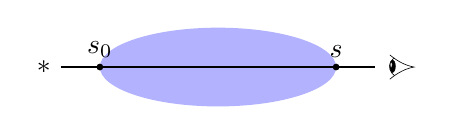
\begin{tikzpicture}
            \fill[blue!30] (0,0) ellipse (1.5 and 0.5);
            \draw (-2,0) -- (2,0) node[left, pos=0]{$*$} node[right,pos=1]{$\text{\lateraleye}$};
            \filldraw[black] (-1.5,0) circle (1pt) node[above] {$s_0$};
            \filldraw[black] (1.5,0) circle (1pt) node[above] {$s$};
        \end{tikzpicture}
    }
    \caption{Luce della stella che passa attraverso il mezzo interstellare.}
    \label{fig:tralenubi}
\end{figure}
Siamo a queste temperature. Consideriamo la sezione d'urto di assorbimento di un atomo in generale:
\[
\sigma = \frac{e^2}{4\epsilon_0m_ec} f \text{ (si trova sul libro)}
\]
Sappiamo inoltre che il coefficiente di assorbimento è legato alla sezione d'urto:
\[
    \alpha_\nu= n\sigma\Phi(\Delta \nu)=\frac{e^2}{4\epsilon_0 M_e c}nf\Phi(\Delta \nu), \quad \int \Phi(\Delta \nu)d\nu = 1.
\]
Noto il coefficiente di assorbimento, possiamo calcolare la profondità ottica, che è ciò che vogliamo ottenere
\[
    \tau_\nu = \int_{s_0}^{s} \alpha(s')ds' = \int_{s_0}^{s}\frac{e^2}{4\epsilon_0 M_e c}nf\Phi(\Delta \nu) ds'= \frac{e^2}{4\epsilon_0 M_e c}f\Phi(\Delta \nu)\int_{s_0}^{s}nds'.
\]
L'ultimo integrale si indica di solito con $N=\int_{s_0}^{s}nds'$ e prende il nome di densità di colonna (degli atomi che assorbono i fotoni con la frequenza della riga). Quindi
\[
    \tau_\nu = \frac{e^2}{4\epsilon_0 M_e c}f\Phi(\Delta \nu) N.
\]
Vogliamo calcolare la larghezza equivalente. Noi sappiamo che l'equazione del trasporto si scrive come 
\[
    \frac{dI_\nu}{ds}=j_\nu-\alpha_\nu I_\nu
\]
Siccome stiamo facendo osservazioni nelle bande del visibile e a queste lunghezze d'onda non ci aspettiamo emissione da un mezzo con $T$ così bassa, scriviamo $j_\nu \approx 0$ nel visibile. Quindi abbiamo
\[
    \frac{dI_\nu}{ds}=-\alpha_\nu I_\nu \quad \Rightarrow \quad  I_\nu(\tau_\nu)=I_\nu(0)e^{-\tau_\nu}
\]
In cui la quantità $I_\nu(0)$ corrisponde all'intensità specifica emessa dalla sorgente prima di entrare nel mezzo, che corrisponde anche all'intensità del del continuo ($I_\nu(0) = I_C$).\\
\begin{center}
    \resizebox{\columnwidth/2}{!}{
        \begin{tikzpicture}
            \pgfplotsset{ticks=none}
                \begin{axis}[   
                    xmin=0,
                    xmax=4,
                    ymin=0,
                    ymax=3,
                    xlabel={$\lambda$},
                    ylabel={$I_\lambda$},
                    xticklabels={,,},
                    yticklabels={,,},
                    scale only axis,
                    axis lines=middle,
                    domain=0:4,
                    samples=250,
                    smooth,
                    clip=false,
                    axis equal image=true,
                    ]
                    \addplot[
                        color=black,
                        domain = 0:4,
                        samples = 100,
                        dashed,
                    ]{2} node[left, pos=0] {$I_C$};
                    \addplot[
                        color=blue,
                        domain = 0:4,
                        samples = 1000,
                    ]{2-1.5*exp(-(x-2)^2/0.05)};
                    \addplot[black,dashed] coordinates { (2, 0) (2, 0.5)};
                    \node at (axis cs:2, 0) [anchor=north]{$\lambda_0$};
                \end{axis}
        \end{tikzpicture}
    }
\end{center}
Possiamo calcolarci la larghezza equivalente:
\[
    W_\lambda = \int\frac{I_C-I_\lambda}{I_C}d\lambda
\]
Convertendo $I_\nu$ in $I_\lambda$ e sostituendo, otterremo
\[
    W_{\lambda_0}=\frac{\lambda_0^2}{c}\int(1-e^{-\tau_\nu})d\nu
\]
Possiamo fare un'ulteriore approssimazione considerando che il mezzo è molto rarefatto. Di conseguenza la riga sarà debole, cioè poco profonda. Questo implica che
\[
    \tau_\nu<<1\quad \Rightarrow\quad e^{-\tau_\nu}\approx1-\tau_\nu
\]
Quindi possiamo scrivere
\[
    W_{\lambda_0}=\frac{\lambda_0^2}{c}\int\tau_\nu d\nu = =\frac{\lambda_0^2}{c}\int \frac{e^2}{4\epsilon_0 M_e c}f\Phi(\Delta \nu) N d\nu.
\]
Risolvendolo, sfruttando il fatto che $ \int \Phi(\Delta \nu)d\nu = 1$, otteniamo
\[
    W_{\lambda_0}=\frac{\lambda_0^2}{c} \frac{e^2}{4\epsilon_0 M_e c}f N d\nu
\]
Di solito si fa un grafico del rapporto 
\[
    \frac{W_{\lambda_0}}{\lambda_0}=\frac{e^2}{4\epsilon_0 M_e c^2} N f \lambda_0
\]
Si scopre quindi che per righe deboli, questo rapporto è proporzionale a $N f \lambda_0$ ed è interessante perché da una misura dell'unica cosa che dipende dalle proprietà della nube, cioè la densità di colonna.\\
Per quello che abbiamo visto, siamo costretti a sfruttare la presenza di stelle che illuminino le nubi (Figure \ref{fig:tralenubi}). Non si era ancora scoperta l'emissione di questo gas. In questo contesto tra 1944 e il 1945, un giovane astronomo e matematico olandese H. van de Hulst, predice l'esistenza di un'emissione prodotta dalle nubi di idrogeno neutro (HI) nel radio, precisamente a $21\um{cm}$. Questa verrà scoperta nel 1951 e da allora è uno degli strumenti diagnostici più importanti per la caratterizzazione del mezzo. Ma perché dovremmo aspettarci un'emissione a 21 cm di HI? Siamo a temperature $T\approx (80\div 100)\um{K}$. Sappiamo che il livello fondamentale dell'idrogeno è splittato in due livelli iperfini, dovuta all'interazione magnetica tra i momenti di dipolo magnetico del nucleo e dell'elettrone in cui la differenza di energia tra i due livelli è $\Delta E = 5.87\times 10^{-6} \um{eV}$.

\begin{wrapfigure}{r}{0pt}
    \centering
    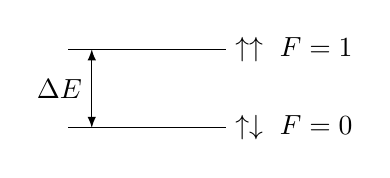
\begin{tikzpicture}
        \draw (0,0) -- (2,0) node[right]{$\uparrow\downarrow\ F=0$};
        \draw (0,1) -- (2,1) node[right]{$\uparrow\uparrow\ F=1$};
        \draw[>=latex, <->, black] (0.3,0) -- (0.3,1) node[left, pos=0.5]{$\Delta E$};
    \end{tikzpicture}
    \caption{Livelli iperfini dell'atomo di idrogeno.}
    \label{fig:livelli_iper}
\end{wrapfigure}
\noindent
 Il livello ad energia più bassa è quello con i due spin antiparallelo, quindi spin del protone e quello dell'elettrone opposto. In questo caso il momento angolare vale $F=0$. Mentre il livello con i due spin paralleli è quello con energia maggiore, in cui il momento angolare vale $F=1$. Quindi il livello più basso non è degenere e quello più alto sarà degenere con degenerazione pari a 3. Se l'atomo si trova nel livello più energetico e si diseccita emettendo un fotone, questo avrà un'energia $\Delta E = h\nu_0$ e facendo i conti si vede che
\[
    \nu_0 = 1.4204\um{GHz} \quad \Rightarrow \quad \lambda_0=21.105\um{cm}
\]
Quanto è probabile questa transizione? La transizione è proibita, quindi la probabilità di emissione spontanea è molto bassa. Infatti il coefficiente di Einstein di questa transizione vale 
\begin{equation}
    A_{10}=2.85\times10^{-15}\um{s}^{-1}.
    \label{eq:a10}
\end{equation}
Il tempo di dimezzamento del livello eccitato è invece molto lungo 
\begin{equation*}
    \tau_{1/2} = \frac{1}{A_{10}}\approx3.5\times10^{14}\um{s} \approx 1.1\times 10^7\um{yr}.
\end{equation*}
Ciò vuol dire che se siamo nel mezzo interstellare, un atomo di idrogeno viene eccitato da una collisione. Il fatto che il mezzo sia molto rarefatto fa sì che non si abbiano diseccitazioni per collisione ma soltanto dopo 11 milioni di anni (in media) avremo una diseccitazione radiativa. Le densità raggiungibili in laboratorio fanno sì che non sia possibile riprodurre il sistema, il che rende il mezzo interstellare un ambiente unico per lo studio di questi fenomeni.\\
Essendo la temperatura così bassa ($T\approx (80\div 100)\um{K}$), siamo sicuri di poter considerare il primo livello (quello eccitato degli iperfini) popolato?
\[
    T=300\um{K},\ kT=\frac{1}{40} \um{eV} \Rightarrow T=100\um{K},\ kT=\frac{1}{120} \um{eV} \gg\Delta E = 5.87\times 10^{-6}\um{eV}
\] 
L'energia termica è molto più grande dell'energia che separa i due livelli iperfini, quindi ci possiamo aspettare che sia popolato.\\
Facciamo una parentesi sull'LTE. Negli interni stellari possiamo considerare il plasma in condizioni di LTE. Ciò vuol dire che il popolamento relativo dei vari livelli energetici è governato dalle collisioni. Mi aspetto che al diminuire della densità, questo cessi di essere vero. Quando questo succede e quindi il nostro gas non è al LTE, bisogna risolvere le equazioni di rate dei processi che popolano e spopolano i livelli energetici. Se non vale LTE non possiamo considerare valide Boltzmann (quindi $\frac{n_2}{n_1}\neq\frac{g_2}{g_1}\exp{(-\frac{h\nu}{kT})}$) e non vale Kirchhoff (quindi $S_\nu \neq B_\nu(T)$). Vediamo cosa succede nel nostro caso specifico.\\
Si definiscono dei coefficienti, analoghi a quelli di Einstein per le reazioni, per le collisioni:
\begin{itemize}
    \item coefficiente di diseccitazione $\gamma_{21}$ tale che il rate di diseccitazione collisionale del livello due sia dato da $\gamma_{21}n_2n_e$.
    \item coefficiente di eccitazione $\gamma_{12}$ tale che il rate di eccitazione collisionale del livello due sia dato da $\gamma_{12}n_1n_e$
\end{itemize}
Immaginiamo di essere in una situazione in cui abbiamo un atomo a due livelli e di considerare sia i processi collisionali che quelli radiativi. Siamo in una condizione stazionaria in cui in media il numero di transizioni $1\to2 = 2\to1$. Il rate di eccitazione sarà dato da
\[
    n_1(B_{12}\Bar{J}+\gamma_{12}n_e)=n_2(A_{21}+B_{21}\Bar{J}+\gamma_{21}n_e)
\]
Vogliamo fare un ragionamento analogo a quello fatto a suo tempo per trovare le relazioni tra i coefficienti. Per farlo avevamo supposto LTE, ma le relazioni trovate restano comunque indipendenti da ciò. Analogamente faremo qui: assumeremo equilibrio termodinamico per calcolare le relazioni ma sappiamo che non c'è bisogno che sia verificato perché le reazioni siano vere.\\

\[
\text{LTE} \Rightarrow J_\nu = I_\nu =B_\nu(T)
\]
Siccome la funzione di Planck varia lentamente in termini di frequenza, nell'intervallo $\Delta\nu$ possiamo considerarla costante, quindi
\[
\Bar{J}\approx B_\nu(T)
\]
Inoltre, siccome siamo in LTE, possiamo scrivere
\[
    \frac{n_2}{n_1}=\frac{g_2}{g_1}e^{-\frac{h\nu}{kT}}
\]
Sostituiamo queste relazioni nelle equazioni di rate e otteniamo
\begin{equation}
    g_1\gamma_{12} = g_2 \gamma_{21} e^{-\frac{h\nu}{kT}}
    \label{rel-gamma}
\end{equation}
Consideriamo il mezzo interstellare. Gli atomi vengono eccitati collisionalmente e consideriamo il caso in cui il mezzo non viene illuminato, cioé consideriamo il caso in cui
\[
    \Bar{J} = 0
\]
Sostituiamo nelle equazioni di prima e otteniamo
\[
n_1 n_e \gamma_{12} =n_2(A_{21}+n_e\gamma_{21})
\]
\[
 \Rightarrow   \frac{n_2}{n_1}=\frac{\gamma_{12}n_e}{A_{21}+\gamma_{21}n_e}
\]
Sostituiamo la relazione tra $\gamma_{12}$ e $\gamma_{21}$ ottenuta in Eq. (\ref{rel-gamma}) e ottengo
\begin{equation*}
     \frac{n_2}{n_1}=\frac{g_2}{g_1}e^{-\frac{h\nu}{kT}}\frac{1}{1+\frac{A_{21}}{\gamma_{21}n_e}}    
\end{equation*}
Se non ci fosse l'ultimo termine avrei ottenuto la relazione di Boltzmann. Quando questo termine va a zero, il popolamento del livello è descritto dalla distribuzione di Boltzmann. Dire che questo termine va a zero implica
\begin{equation}
    \frac{A_{21}}{\gamma_{21}n_e}\ll 1 \Rightarrow A_{21} \ll n_e\gamma_{21}
    \label{eq:limite_bol}
\end{equation}
Cioè stiamo dicendo che, nel limite in cui la probabilità di diseccitazione radiativa diventa trascurabile rispetto a quella collisionale, ricadiamo nella distribuzionedi Boltzmann. Infatti sappiamo che in LTE il popolamento dei livelli è determinato dalle collisioni. \\
Quando vale la relazione Eq. (\ref{eq:limite_bol})? Quando si raggiunge una densità critica
\[
    n_{e,c} = \frac{A_{21}}{\gamma_{21}}
\]
Quando $n_e\gg n_{e,c} $ siamo in LTE, altrimenti no.\\
Per le transizioni permesse, il coefficiente $A_{21}$ sarà grande, quindi anche la densità critica mentre quella del mezzo sarà più piccola rispetto alla crititca. Non potremo quindi considerare il mezzo in LTE. Nel caso della reazione a 21cm abbiamo visto che $A_{21}$ è molto picocolo (Eq.(\ref{eq:a10})), e la densità critica vale
\begin{equation}
    \text{HI } 21\um{cm} \to n_c\approx3\times10^{-5}\um{cm}^{-3}
\end{equation}
Che è minore della densità delle nubi di HI ($\sim (1\div100)\um{cm}^{-3}$. Tuttavia riusciamo a vedere l'emissione delle nubi a 21 cm ma non riusciamo a farlo in laboratorio. Infatti in un qualsiasi laboratorio abbiamo densità molto più grandi rispetto a quella delle nubi. Inoltre in una nube abbiamo un'enorme quantità di atomi di idrogeno. Quindi per quanto sia un evento molto raro, questi due aspetti fanno sì che ci sia un'emissione che produce un segnale importante.\\
Ora vogliamo calcolare la riga di emissione spontanea dell'idrogeno neutro a 21 cm. Calcoliamo innanzitutto il popolamento dei livelli, cioè $n_2/n_1$
\[
\text{LTE} \Rightarrow     \frac{n_2}{n_1}=\frac{g_2}{g_1}e^{-\frac{h\nu}{kT}}
\]
Sappiamo che per $T=80K$, $h\nu = 5.87\times10^{-6}\um{eV}\ll kT=6.9\times10^{-3}\um{eV}$ e quindi che $e^{-\frac{h\nu}{kT}}\ll1$, il che implica che
\[
\frac{n_2}{n_1}\approx\frac{g_2}{g_1}=3
\]
L'ultima uguaglianza è dovuta al fatto che il livello 2 ha degenerazione uguale a 3, mentre il livello 1 non ha degenerazione, quindi è uguale a 1. Quindi, siccome le temperature tipiche delle nubi interstellari garantiscono un'energia termica che è diversi ordini di grandezza più grande della differenza di energia fra i livelli, il rapporto tra il popolamento dei livelli è indipendente dalla temperatura.\\
Sappiamo che 
\[
    \begin{cases}
        n_1+n_2 = n_\text{H}\\
        n_2/n_1=3
    \end{cases}
    \Rightarrow
    \begin{cases}
        n_1=\frac{n_\text{H}}{4}\\
        n_2=\frac{3}{4}n_\text{H}
    \end{cases}
\]
Abbiamo un mezzo rarefatto, vogliamo studiare l'emissione del mezzo non retroilluminato, quindi andiamo a riprendere la soluzione dell'equazione del trasporto 
\[
    I_\nu(\tau_\nu)=I_0(\nu)e^{-\tau_\nu}+\int_{0}^{\tau_\nu}e^{-(\tau_\nu-\tau_\nu')}S_\nu(\tau_\nu')d\tau_\nu'
\]
E dato che il mezzo non è retroilluminato $I_\nu(0)=0$. In caso di mezzo omogeneo avremmo 
\[
    I_\nu(\tau_\nu)=S_\nu(1-e^{-\tau_\nu})
\]
Ci aspettiamo che essendo rarefatto, il mezzo sia otticamente sottile
\[
    \tau_\nu\ll1\Rightarrow I_\nu(\tau_\nu) = j_\nu L
\]
Nel nostro caso non possiamo considerare il mezzo omogeneo, per cui
\[
    I_\nu(\tau_\nu)\approx \int j_\nu ds
\]
e abbiamo bisogno dell'intensità su tutto il profilo
\[
I=\int I_\nu d\nu = \int ds \int j_\nu d\nu
\]
In pratica, se conoscessimo la forma di $j_\nu$ potremmo calcolare l'intensità della riga. Ma in realtà possiamo calcolarlo, infatti 
\[
    j_\nu = \frac{h\nu_0}{4\pi}n_2A_{21}\Phi(\Delta \nu)
\]
E a questo punto lo sostituiamo e integriamo, ottenendo
\[
    I = \frac{h\nu_0}{4\pi}A_{21}\int n_2 ds
\]
Dove come al solito abbiamo sfruttato il fatto che $\int \Phi(\Delta \nu)d_\nu = 1$. Sapendo che $n_2=\frac{3}{4}n_\text{H}$, abbiamo
\[
    I = \frac{3}{16\pi}h\nu_0A_{21}\int n_\text{H} ds = \frac{3}{16\pi}h\nu_0A_{21} N_{\text{HI}}
    \label{eq:intemi}
\]
Con $N_\text{HI}$ densità di colonna dell'idrogeno neutro. È fondamentale osservare che l'intensità di emissione dipende dalla densità di colonna ma non dipende dalla temperatura! Ce lo aspettiamo poiché l'emissione spontanea dipende da $n_2$ che non dipende dalla temperatura. Il tutto perché $kT$ è enorme rispetto ad $h\nu$. Si fanno osservazioni nel radio, si misura l'intensità dalle righe, il coefficiente di Einstein lo conosciamo dalle misure di laboratorio e questo ci da una stima della densità di colonna. \\
Per caratterizzare completamente il mezzo ci sarebbe bisogno di misurare la densità della riga di assorbimento. Per farlo mettiamo una sorgente dietro il mezzo (\ref{fig:tralenubi}) e calcoliamo l'intensità:
\[
 I_\nu = I_\nu(0)e^{-\tau_\nu},
\]
con
\begin{equation}
    \tau_\nu = \int_{s_0}^{s}\alpha_\nu(s')ds'.
    \label{eq:prottica}
\end{equation}
Per caclcolare la profondità ottica dobbiamo conoscere il coefficiente di assorbimento
\[
    \alpha_\nu= \frac{h\nu}{4\pi}\Phi(\Delta\nu)\left[ n_1B_{12}-n_2B_{21}\right]
\]
Notare il termine dovuto all'emissione stimolata. Nelle bande ottiche lo abbiamo trascurato, poiché gli atomi del mezzo erano nel fondamentale e non c'erano atomi che potessero emettere nell'ottico con l'emissione stimolata. Qui conta e, come abbiao visto, possiamo riscriverlo come
\begin{equation}
    \alpha_\nu= \frac{h\nu}{4\pi}\Phi(\Delta\nu)n_1B_{12}\left[1 -e^{-\frac{h\nu}{kT}}\right]
    \label{eq:assorbimento}
\end{equation}
Nel visibile avevamo $h\nu$ grande rispetto a $kT$, ma a 21cm $h\nu\ll kT$, quindi $e^{-\frac{h\nu}{kT}}\approx 1-\frac{h\nu}{kT}$ e riscriviamo la \ref{eq:assorbimento} come
\begin{equation}
    \alpha_\nu= \frac{h\nu}{4\pi}\Phi(\Delta\nu)n_1B_{12}\frac{h\nu}{kT}
\end{equation}
Ora esprimiamo il coefficiente di assorbimento in termini di emissione spontanea sfruttando le relazioni
\begin{gather*}
    g_1B_{12}=g_2B_{21}\\
    A_{21}=\frac{2h}{c^2}\nu^3B_{21}\\
    n_1=\frac{n_\text{H}}{4}\\
    \frac{g_2}{g_1}=3
\end{gather*}
e otteniamo
\begin{equation}
    \alpha_\nu = \frac{3}{32\pi}\frac{hc^2}{kT}n_\text{H}A_{21}\frac{\Phi(\Delta\nu)}{\nu}
\end{equation}
A questo punto si ha la profondità ottica dalla \ref{eq:prottica} e otteniamo
\begin{equation}
    \tau_\nu = \frac{3}{32\pi}\frac{hc^2}{k}A_{21}\frac{\Phi(\Delta\nu)}{\nu}\int\frac{n_\text{H}}{T}ds
\end{equation}
Notiamo che la profondità ottica e quindi la riga di assorbimento dipendono anche dalla temperatura, a differenza della riga di emissione. Più alta è la temperatura più il mezzo è trasparente e più debole sarà la riga. \\
Con l'osservazione della riga a 21 cm si sono ottenute le prime evidenze che le nubi di gas non sono distribuite uniformemente sul disco ma a bracci di spirale.\\
\begin{figure}[t!]
    \centering
    \resizebox{.8\columnwidth}{!}{%
        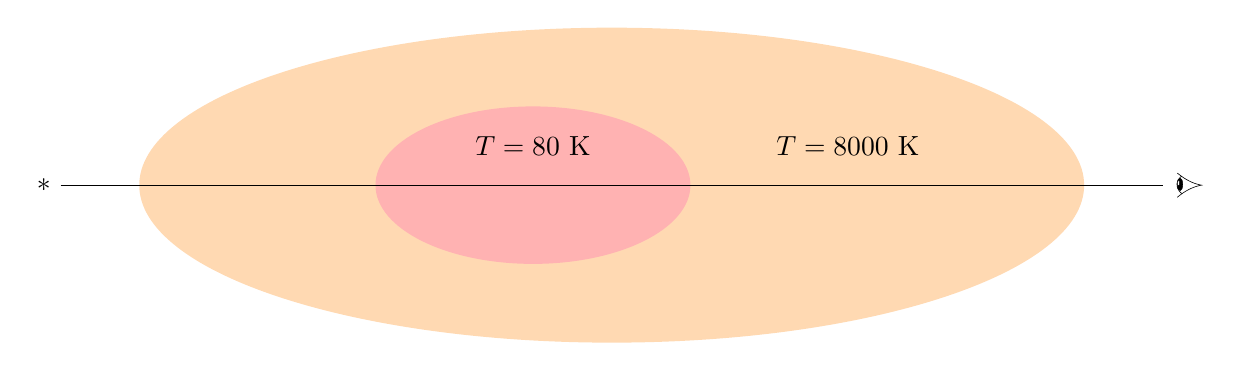
\begin{tikzpicture}
            \fill[orange!30] (0,0) ellipse (6 and 2);
            \fill[red!30] (-1,0) ellipse (2 and 1);
            \draw (-7,0) -- (7,0) node[left, pos=0]{$*$} node[right,pos=1]{$\text{\lateraleye}$};
            \node(hot) at (3,.5){$T=8000\um{K}$};
            \node(cold) at (-1,.5){$T=80\um{K}$};
        \end{tikzpicture}
    }
    \caption{Temperature delle nubi di idrogeno.}
    \label{fig:nubitemp}
\end{figure}
Lo studio della differente dipendenza da temperatura e densità nei casi di emissione ed assorbimento fece scoprire che oltre alla componente di idrogeno fredda ce ne fosse anche una calda (Fig.\ref{fig:nubitemp}). Il mezzo è composto per la maggior parte (in massa) dalla zona fredda, mentre la parte calda è molto rarefatta. La densità della zona fredda è circa $(1\div100)\um{cm}^{-3}$, mentre di quella calda è circa $(0.1\div1)\um{cm}^{-3}$.\\
\begin{figure}[b!]
    \centering
    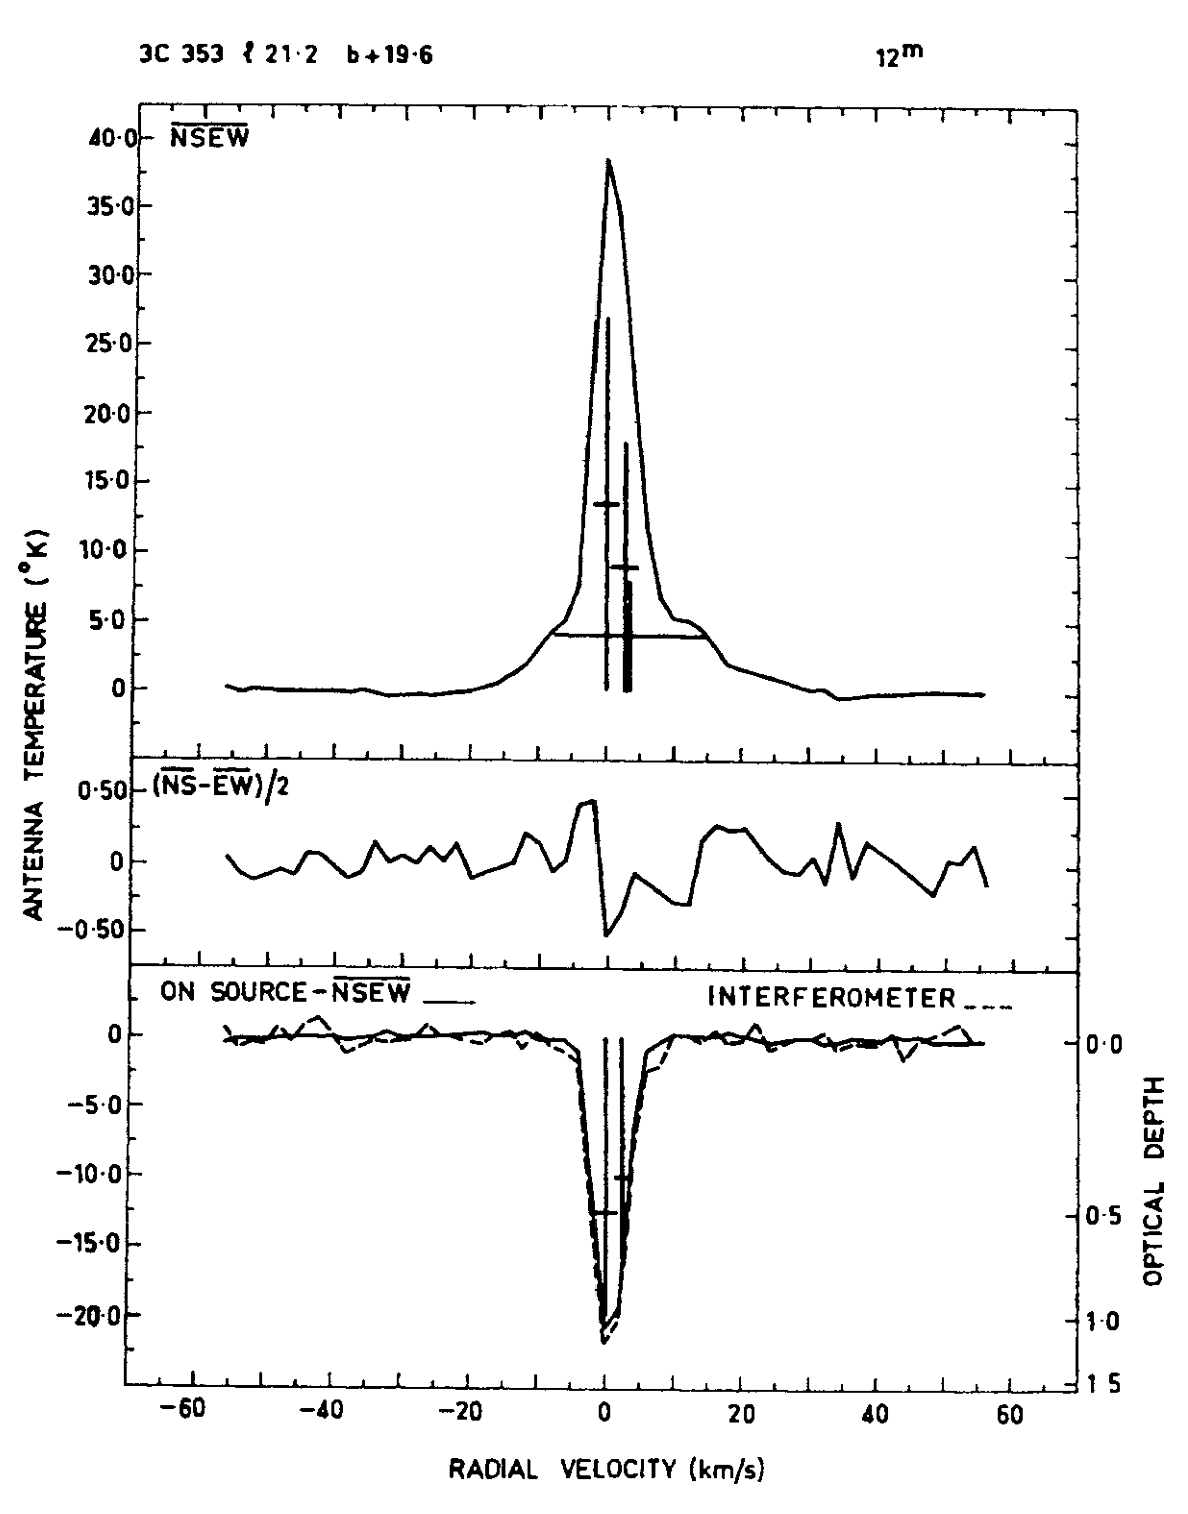
\includegraphics[width=.4\columnwidth]{images/assoemi.png}
    \caption{Riga di emissione a 21 cm del mezzo interstellare nel (sopra) e la riga di assorbimento a 21 cm prodotta dal mezzo interstellare (sotto). Sorgente 3C 353.}
    \label{fig:assoemi}
\end{figure}
Un mezzo fatto come in Figura \ref{fig:nubitemp} produce righe di assorbimento ed emissione a 21 cm come nella Figura \ref{fig:assoemi}. Abbiamo visto nell'Eq. \ref{eq:intemi} che l'intensità della riga di emissione dipende solo dalla densità di colonna, quindi in particolare significa che è indipendente dalla temperatura. Quando andiamo ad osservare abbiamo che parte della riga sarà data dalla nube fredda e parte da quella calda. Se la densità di colonna lungo la linea di vista è confrontabile per il mezzo alle diverse temperature, la riga avrà due contributi che hanno intensità confontabile. Tuttavia la larghezza di questi contributi deve essere diversa: più larga in quella della zona calda, più stretta in quella della fredda. Ed è questo che notiamo guardando la Figura \ref{fig:assoemi}, in cui la riga di emissione ala base è larga e poi si stringe. è la sovrapposizione di due righe. Nella riga di assorbimento la situazione è diversa, dato che questa dipende dalla temperatura. Dato che la profondità ottica diminuisce con l'aumento della temperatura, l'intensità della riga di assorbimento prodotta nella zona calda sarà molto più debole di quella della zona fredda. Gran parte della riga è prodotta quindi nella zona fredda ed ha la larghezza di una riga ad $80\um{K}$ e non $8000\um{K}$.\\
Oltre a polvere ed idrogeno neutro, nel mezzo interstellare sono presenti delle nubi molecolari, le cui caratteristiche principali sono $n\approx 10^3\um{cm}^{-3}$, $T=10\div30\um{K}$. Queste sono composte principalmente da molecole di $\ce{H2}$. Sono difficili da osservare non avendo emissioni nel radio. Si possono osservare nell'ultravioletto se c'è una sorgente che le illumina. Per caratterizzarne la distribuzione geometrica non si usano le molecole di idrogeno, ma di molecole di $\ce{CO}$, anche queste abbastanza abbondanti. Queste hanno un'emissione molto intensa dovuta alle transizioni rotazionali a $\lambda =2.6\um{mm}$ che corrisponde a $\nu_0 = 115\um{GHz}$. Inoltre sono osservabili anche i multipli $2\nu_0,3\nu_0,\dots,n\nu_0$.\\
Una cosa interessante delle nubi molecolari è che si è scoperta la presenza di molecole di molti tipi diversi, tra cui anche molecole organiche (addirittura amminoacidi). E da queste molecole sono state scoperte intensità di emissione molto elevate che se fosse dovuta ad emissione termica per giustificarla avremmo bisogno di temperature di miliardi di gradi. In realtà si è scoperto che l'intensità così elevata non è da attribuire all'emissione termica ma all'inversione di popolazione dei livelli energetici che è più facile da ottenere per le molecole rispetto agli elementi. Si ha un'emissione non termica ma MASER. Nel cosmo ci sono molti fenomeni e molte molecole che producono MASER (OH, CH, SiO, $\ce{NH3}$, $\ce{H2O}$, HCN). Ciò che produce il pompaggio che determina l'inversione di popolazione è di solito un'intensa radiazione nell'infrarosso, a sua volta prodotta dalla polvere riscaldata da qualche tipo di processo (ad esempio, in scale piccole, nelle nubi stellari).
\newpage
\section*{20-05 - Galassie2}
\subsection*{Struttura della galassia}
\begin{figure}[h]
    \centering
    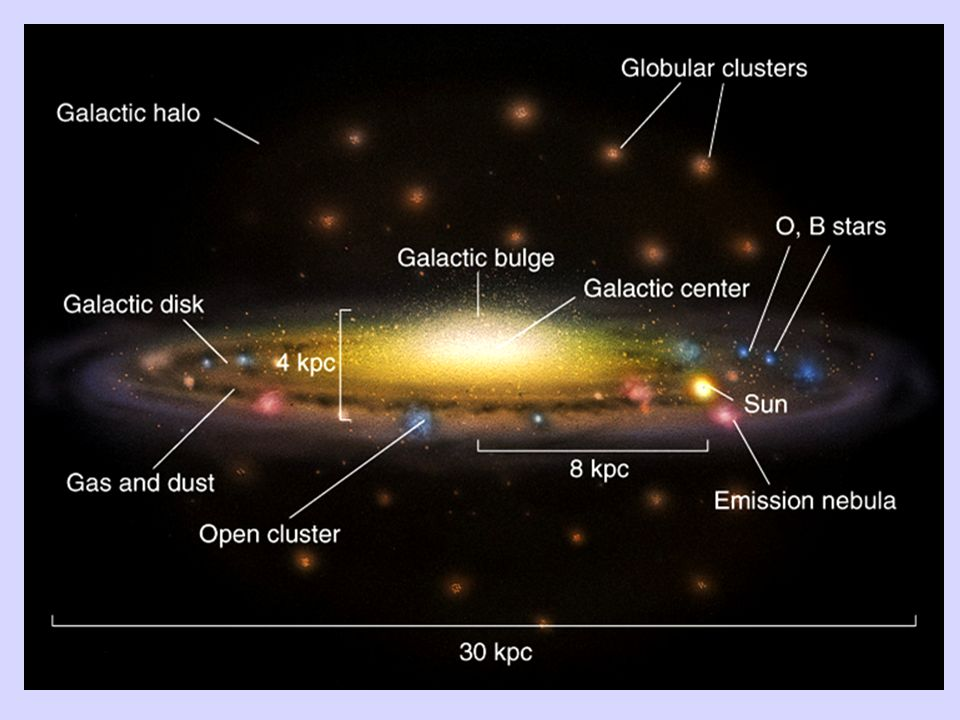
\includegraphics[width=.8\columnwidth]{images/strutturagalassia.jpg}
    \caption{Principali strutture di una galassia.}
    \label{fig:strutturagalassia}
\end{figure}
\noindent
Nella Figura \ref{fig:strutturagalassia} vediamo una rappresentazione della Via Lattea in cui sono indicate le principali strutture che la compongono. Il disco, cioè la parte più sottile, ha un raggio dell'ordine di 20 kpc. Come si può immaginare, è difficile parlare di estensione poiché nel punto in cui finiscono le stelle ci sono ancora diversi kpc in cui si estendono i gas del ISM. Sul disco abbiamo stelle di diverse generazioni ed il ISM (polvere, HI e nubi molecolari). La zona sferoidale è chiamata alone, dove troviamo gli ammassi globulari. Si distingue dal disco perché le stelle che lo popolano sono solo antiche ($\gtrsim 10^{10}\um{yr}$) e sono tutte povere di metalli. Le stelle che hanno queste caratteristiche prendono il nome di stelle di Popolazione 2. Le altre prendono il nome di stelle di popolazione 2. Nella zona centrale troviamo il bulge, un rigonfiamento che ha un raggio dell'ordine del kpc. Ha una grande densità di stelle vecchie e ricche di metallo e di ISM.\\

\subsection*{Contributo di gas ionizzato - Nubi di HII}
Dobbiamo aspettarci il contributo di un gas ionizzato. Sappiamo che le stelle nascono dalla contrazione delle nubi di gas interstellare. Una volta che accendiamo la stella, cosa succede al gas che la circonda?\\
Sappiamo che l'energia per ionizzare l'idrogeno neutro $\ce{HI}$ deve essere $E\ge E_0=13.6\um{eV}$. A quest'energia corrisponde una $\lambda\le\lambda_0 = 912$ \AA. Le stelle emettono un numero significativo di fotoni con questa lunghezza d'onda? Dipenderà dalla temperatura effettiva. Guardando i tipi spettrali, scopriamo che le stelle in grado di produrre fotoni in grado di ionizzare l'HI sono quelle di tipo O e di tipo B ($T_{\text{eff}}>20000\um{K}$). Sappiamo che nel gas abbiamo anche He ma l'energia di prima ionizzazione dell'elio è abbastanza più alta da rendere la sua ionizzazione decisamente più rara (sono poche le stelle abbastanza massicce). Avremo un processo del tipo
\[
    \ce{HI + {\gamma}  -> HII + e-}
\]

\begin{figure}[h!]
    \centering
    \resizebox{.4\columnwidth}{!}{%
        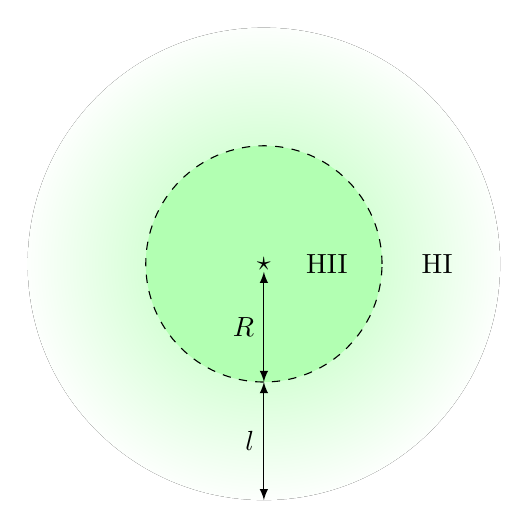
\begin{tikzpicture}
            \fill[even odd rule,inner color=green!30,outer color=green!1] (0,0) circle (3);
    %        \fill[blue!5] (0,0) circle (3);
            \filldraw[fill=green!30,dashed] (0,0) circle (1.5);
            % \filldraw[black] (0,0) circle (1pt) node[above] {Star};
            \draw[>=latex, <->, black] (0,-0.1) -- (0,-1.5) node[left, pos=.5]{$R$};
            \draw[>=latex, <->, black] (0,-1.5) -- (0,-3) node[left, pos=0.5]{$l$};
            \node(h1) at (.8,0){HII};
            \node(h2) at (2.2,0){HI};
            \node(stella) at (0,0){$\star$};
        \end{tikzpicture}
    }
    \caption{Distribuzione dell'idrogeno attorno ad una stella.}
    \label{fig:idrogenostelle}
\end{figure}
Vogliamo sapere quanto è grande la regione HII (vedi Figura \ref{fig:idrogenostelle}). Il primo a studiare questo tipo di processo fu Strongren nel 1939. Fece due assunzioni: la stella, massiccia, arriva molto rapidamente alla fase di sequenza principale (che non è vero, sappiamo che ci vogliono decine di migliaia di anni), e che il mezzo che circondava la stella appena nata è omogeneo. Con queste due assunzioni, la regione prende una forma sferica che prende il nome di Sfera di Strongren. Supponiamo che ad un certo istante la stella abbia ionizzato la regione di raggio $R$. Un fotone ionizzante emesso dalla stella attraverserà la zona già ionizzata praticamente indisturbatamente. Vediamo perché. In questa regione abbiamo soltanto protoni ed elettroni, quindi il tipo di interazione tra fotone e mezzo sarà di scattering elettronico. Sappiamo che a queste energie saremo nel limite non relativistico e che quindi avremo uno scattering Thomson, che è molto piccola ($\sigma_\text{T}=6.65\times10^{-25}\um{cm}^2$). Il cammino libero medio di un fotone ionizzante sarà
\begin{equation}
    l_\text{T} = \frac{1}{n_e\sigma_\text{T}} \gg R
\end{equation}
dato che $n_e\sim n_\text{H}\approx10^3\um{cm}^{-3}$ e che quindi $l_\text{T}\approx10 \um{pc}$. Di conseguenza il fotone ionizzante entra nella zona di HI, in cui invece ha una sezione d'urto $\sigma \approx 10^{-17}\um{cm}^2$ e quindi $l=\frac{1}{n_\text{HI}\sigma}\approx 10^{-3}\um{pc}$. Quindi questo fotone non riuscirà mai ad uscire dalla regione di HI. Quindi per ogni fotone ionizzante prodotto si avrà una ionizzazione nella regione di idrogeno neutro, che produce uno spostamento del fronte di ionizzazione, sta aumentando $R$. Fino a quando aumenterà? Presa una shell di raggio $dR$, avremo un numero di atomi nella shell pari a 
\begin{equation}
    dN_\text{H} = 4\pi R^2 n_\text{HI} dR
\end{equation}
Di quanto riuscirà a progredire il fronte di ionizzazione dipernderà dal numero di fotoni ionizzanti emessi nell'unità di tempo. Sapendo che ciascun fotone ionizzante ionizzerà un atomo di idrogeno possiamo scrivere 
\begin{equation}
    dN_i= dN_\text{H} \Rightarrow \frac{dN_i}{dt} = 4\pi R^2 n_\text{HI} \frac{dR}{dt}.
    \label{eq:ionizzanti}
\end{equation}
Questa situazione non può andare avanti in eterno. Prima o poi gli atomi che si trovano nella regione ionizzata HII si ricombineranno e formeranno di nuovo un atomo di idrogeno neutro. Quando questo succederà l'Eq. \ref{eq:ionizzanti} non sarà più valida perché i fotoni prodotti dalla stella verranno intercettati dagli atomi ricombinati. Di conseguenza dobbiamo aggiungere un altro termine che tenga conto dei fotoni intercettati. Se conosciamo il rate di ricombinazione ($r=n_pn_e\alpha$), scriviamo
\begin{equation}
    \frac{dN_i}{dt} = 4\pi R^2 n_\text{HI} \frac{dR}{dt}+ \frac{4}{3}\pi R^3 n_pn_e\alpha
    \label{eq:ricombinati}
\end{equation}
con $\alpha=\langle\sigma_rv\rangle$, in cui $\sigma_r$ è la sezione d'urto della ricombinazione. Man mano che la sfera aumenta di raggio crescerà tanto il termine di destra fino a diventare dominante. Quando ciò avviene deve succedere
\begin{equation}
    \frac{dR}{dt}=0 \Rightarrow \frac{dN_i}{dt}=\frac{4}{3}\pi R_\text{S}^3 n_pn_e\alpha
\end{equation}
e la zona non può più aumentare di raggio. $R_\text{S}$ prende il nome di raggio di Strongren e, riscrivendo, vale
\begin{equation}
    R_\text{S}=\left(\frac{3}{4\pi n_pn_e\alpha}\frac{dN_i}{dt}\right)^{\frac{1}{3}}.
\end{equation}
Le dimensioni di questo raggio dipenderanno dalla stella, particolarmente dal numero di fotoni ionizzanti e quindi dalla luminosità ad una certa frequenza. Scriviamo che
\begin{equation}
    \frac{dN_i}{dt} = \int_{\nu_{0}}^{\infty} \frac{L_\nu}{h\nu}d\nu,\quad h\nu=13.6\um{eV}
\end{equation}
Quindi se conosciamo lo spettro della stella possiamo calcolare quanti fotoni hanno l'energia sufficiente a ionizzare un atomo di idrogeno e quindi calcolare il raggio della zona HII. Per curiosità, una stella di tipo O5V produce ${dN_i}/{dt}\approx 3\times10^{49}\um{s}^{-1}$.\\
Continua pag. 185 Choudhuri con bremsstrahlung e gas coronale.
\end{document}
